\documentclass{article}
% if you need to pass options to natbib, use, e.g.:
%     \PassOptionsToPackage{numbers, compress}{natbib}
% before loading neurips_2023
\PassOptionsToPackage{numbers,compress}{natbib}
\usepackage[final]{neurips}
% to avoid loading the natbib package, add option nonatbib:
%    \usepackage[nonatbib]{neurips}


\usepackage[utf8]{inputenc} % allow utf-8 input
\usepackage[T1]{fontenc}    % use 8-bit T1 fonts
\usepackage{hyperref}       % hyperlinks
\usepackage{url}            % simple URL typesetting
\usepackage{booktabs}       % professional-quality tables
\usepackage{amsfonts}       % blackboard math symbols
\usepackage{amsmath}        % mathematical environments
\usepackage{nicefrac}       % compact symbols for 1/2, etc.
\usepackage{microtype}      % microtypography
\usepackage{xcolor}         % colors
\usepackage{graphicx}       % figures and image scaling
\usepackage{float}          % H float placement

\title{VAE vs. Pixel and Latent Diffusion: Quality–Compute Trade-offs in Apparel Image Generation}

\author{%
  Yuye Huang\\
  Department of Electrical and Computer Engineering\\
  University of Toronto\\
  \texttt{yuye.huang@mail.utoronto.ca} \\
  \And
  Jenny You\\
  Department of Mechanical and Industrial Engineering\\
  University of Toronto\\
  \texttt{Jenny.You@mail.utoronto.ca} \\
  \And
  Jasmine Shao\\
  Department of Mechanical and Industrial Engineering\\
  University of Toronto\\
  \texttt{jasmine.shao@mail.utoronto.ca} \\
}

\begin{document}

\maketitle

\begin{abstract}
We study the trade-off between generation quality and computational efficiency in three generative image models: a spatial variational autoencoder (VAE), a pixel-space denoising diffusion probabilistic model (DDPM), and a latent diffusion model (LDM). The models are evaluated on Fashion-MNIST and an imbalanced 15-class color-apparel dataset using five independent seeds per model--dataset pair. A frozen task-specific classifier provides feature-based and semantic evaluation metrics. Pixel DDPM achieves the best feature FID on both datasets ($29.64\pm1.49$ and $16.67\pm0.85$), while LDM retains stronger recognizability with 13.9$\times$ faster sampling. VAE is approximately 292$\times$ faster than DDPM but produces the largest distribution mismatch. These results show a consistent quality--compute frontier: pixel diffusion provides the strongest fidelity, latent diffusion offers a more efficient quality compromise, and VAE prioritizes speed over distributional accuracy.
\end{abstract}

\section*{Attestation of Teamwork}
All members contributed to the project design, experimental planning, interpretation, and final integration. Jenny focused on the VAE implementation and latent-space experiments; Yuye on DDPM training, sampling, and denoising analysis; and Jasmine on the shared evaluation pipeline, quantitative analysis, model comparison, and report preparation. The LDM implementation, second-dataset extension, multi-seed experiments, and final conclusions were jointly reviewed and integrated.

\section{Introduction} 

A VAE samples from a learned latent representation and decodes in one pass \citep{kingma2014vae}; a pixel-space DDPM generates through iterative denoising \citep{ho2020ddpm}; and an LDM performs the same process in a compressed latent space \citep{rombach2022ldm}. These differences create trade-offs between generation quality and computational efficiency. 

We compare the three systems on balanced Fashion-MNIST and a smaller, imbalanced color-apparel dataset to answer two questions: how do they trade generation quality against compute, and do these rankings remain consistent across datasets? Each model is evaluated over five independent seeds using a common $32\times32$ interface, 5,000 generated samples, and a frozen task-specific evaluator for each dataset. Hyperparameters are selected using training-derived validation data only, making this a controlled system-level comparison of the three generative pipelines.

\section{Preliminaries and Problem Formulation}

Let $x\sim p_{\mathrm{data}}(x)$ denote an apparel image. The VAE is trained with the reconstruction--regularization objective
\begin{equation}
\mathcal{L}_{\mathrm{VAE}}
=
-\mathbb{E}_{q_\phi(z\mid x)}[\log p_\theta(x\mid z)]
+
\beta D_{\mathrm{KL}}
\!\left(q_\phi(z\mid x)\,\|\,\mathcal{N}(0,I)\right).
\end{equation}
Both diffusion systems use the cosine forward process \citep{nichol2021improved} and noise-prediction objective
\begin{equation}
x_t=\sqrt{\bar{\alpha}_t}x_0+\sqrt{1-\bar{\alpha}_t}\epsilon,
\qquad
\mathcal{L}_{\mathrm{simple}}
=
\mathbb{E}\|\epsilon-\epsilon_\theta(x_t,t)\|_2^2.
\end{equation}
Pixel DDPM applies this objective directly to $3\times32\times32$ images, whereas LDM applies it to standardized $4\times8\times8$ VAE latents.


\section{Design}

\subsection{Datasets and controlled interface}

Fashion-MNIST contains 60,000 training and 10,000 test images from ten balanced clothing classes \citep{xiao2017fashion}. Images are resized from $28\times28$ to $32\times32$ and replicated to three channels. For the color domain, we use the 15 most frequent Apparel classes from Fashion Product Images Small \citep{fpis}, producing a deterministic stratified 85/15 split with 8,007 training and 1,423 test images. Images are center-padded before resizing, and the resulting dataset introduces class imbalance and greater visual variation in color, texture, pose, and background.

\subsection{Model design}

All generators use residual convolutional blocks, while both diffusion models use time-conditioned U-Nets with skip connections and bottleneck self-attention. The LDM reuses the VAE's spatial latent representation, reducing diffusion from 1,024 pixel locations to 64 latent locations. Table~\ref{tab:configuration} summarizes the structural differences relevant to the comparison.

\begin{table}[H]
\caption{Principal architectural and sampling differences. LDM parameter count includes its VAE.}
\label{tab:configuration}
\centering
\small
\begin{tabular}{lccc}
\toprule
Setting & VAE & Pixel DDPM & LDM \\
\midrule
Sampling space
& $4\!\times\!8\!\times\!8$ latent
& $3\!\times\!32\!\times\!32$ pixels
& $4\!\times\!8\!\times\!8$ latent \\

Core network
& Encoder--decoder
& Time-conditioned U-Net
& VAE $+$ latent U-Net \\

Sampling
& One decode
& 100 reverse steps
& 100 latent steps $+$ decode \\

Parameters
& 1.955M
& 5.787M
& 7.743M \\
\bottomrule
\end{tabular}
\end{table}

For each dataset, a residual CNN trained on real data is frozen as the evaluator, providing 256-dimensional task-specific features \citep{he2016resnet}.

\section{Methodology}

\subsection{Training and sampling}
Models use AdamW \citep{loshchilov2019adamw} with batch size 256 and cosine learning-rate decay. The VAE is trained for 3,000 updates, while both diffusion models use 5,000 updates, 100 reverse steps, and EMA parameter averaging. LDM operates in standardized $4\times8\times8$ latents, reducing spatial positions by 16$\times$ relative to pixel space. Full configurations and stabilization choices are provided in Appendix~\ref{app:tuning}.

\subsection{Validation and model selection}
Hyperparameters are selected only from training-derived validation data, with generator settings chosen on Fashion-MNIST and transferred unchanged to the color dataset. Official test sets are reserved for final evaluation; search spaces and selected configurations are reported in Appendix~\ref{app:tuning}.

\subsection{Evaluation}
Using the corresponding frozen evaluator, we measure feature-distribution similarity with FID \citep{heusel2017fid} and KID \citep{binkowski2018kid}, class-proportion agreement with JSD, recognizability and class balance with classifier-based statistics, and efficiency with training time, sampling time, parameter count, and peak GPU memory. Additional diagnostics are reported in the appendix.


\section{Numerical Experiments}
\subsection{Implementation and evaluator reliability}
Experiments run in PyTorch 2.11 with CUDA 12.8 on an RTX 5070 Ti. Native BF16, pinned-memory loaders, persistent workers, cuDNN benchmarking, and a 4,096-image diffusion sampling batch improve throughput. Exact-shape warm-ups and CUDA synchronization isolate steady-state timing. Every central value is a mean over seeds 0--4 and uncertainty is sample standard deviation.

The final Fashion-MNIST evaluator achieves 94.23\% accuracy and balanced accuracy; Shirt is the hardest class at 79.90\% recall. The color evaluator achieves 88.05\% accuracy but 77.40\% balanced accuracy, a 10.65-point gap; rare Sweaters, Jackets, and Sweatshirts have only 31.82\%, 40.00\%, and 45.45\% recall. Class weighting raises minimum validation recall from 25.00\% to 41.67\% but lowers the predefined combined selection score from 84.81\% to 84.60\%, so the unweighted evaluator is retained and both accuracy measures are disclosed. Generated-label metrics on the color set are therefore evaluator-relative rather than ground truth. Appendix~\ref{app:evaluator} reports the confusion matrices, per-class recall, and test-set imbalance.

\subsection{Distribution fidelity}

\begin{figure}[ht]
\centering
\begin{minipage}{0.47\linewidth}
  \centering
  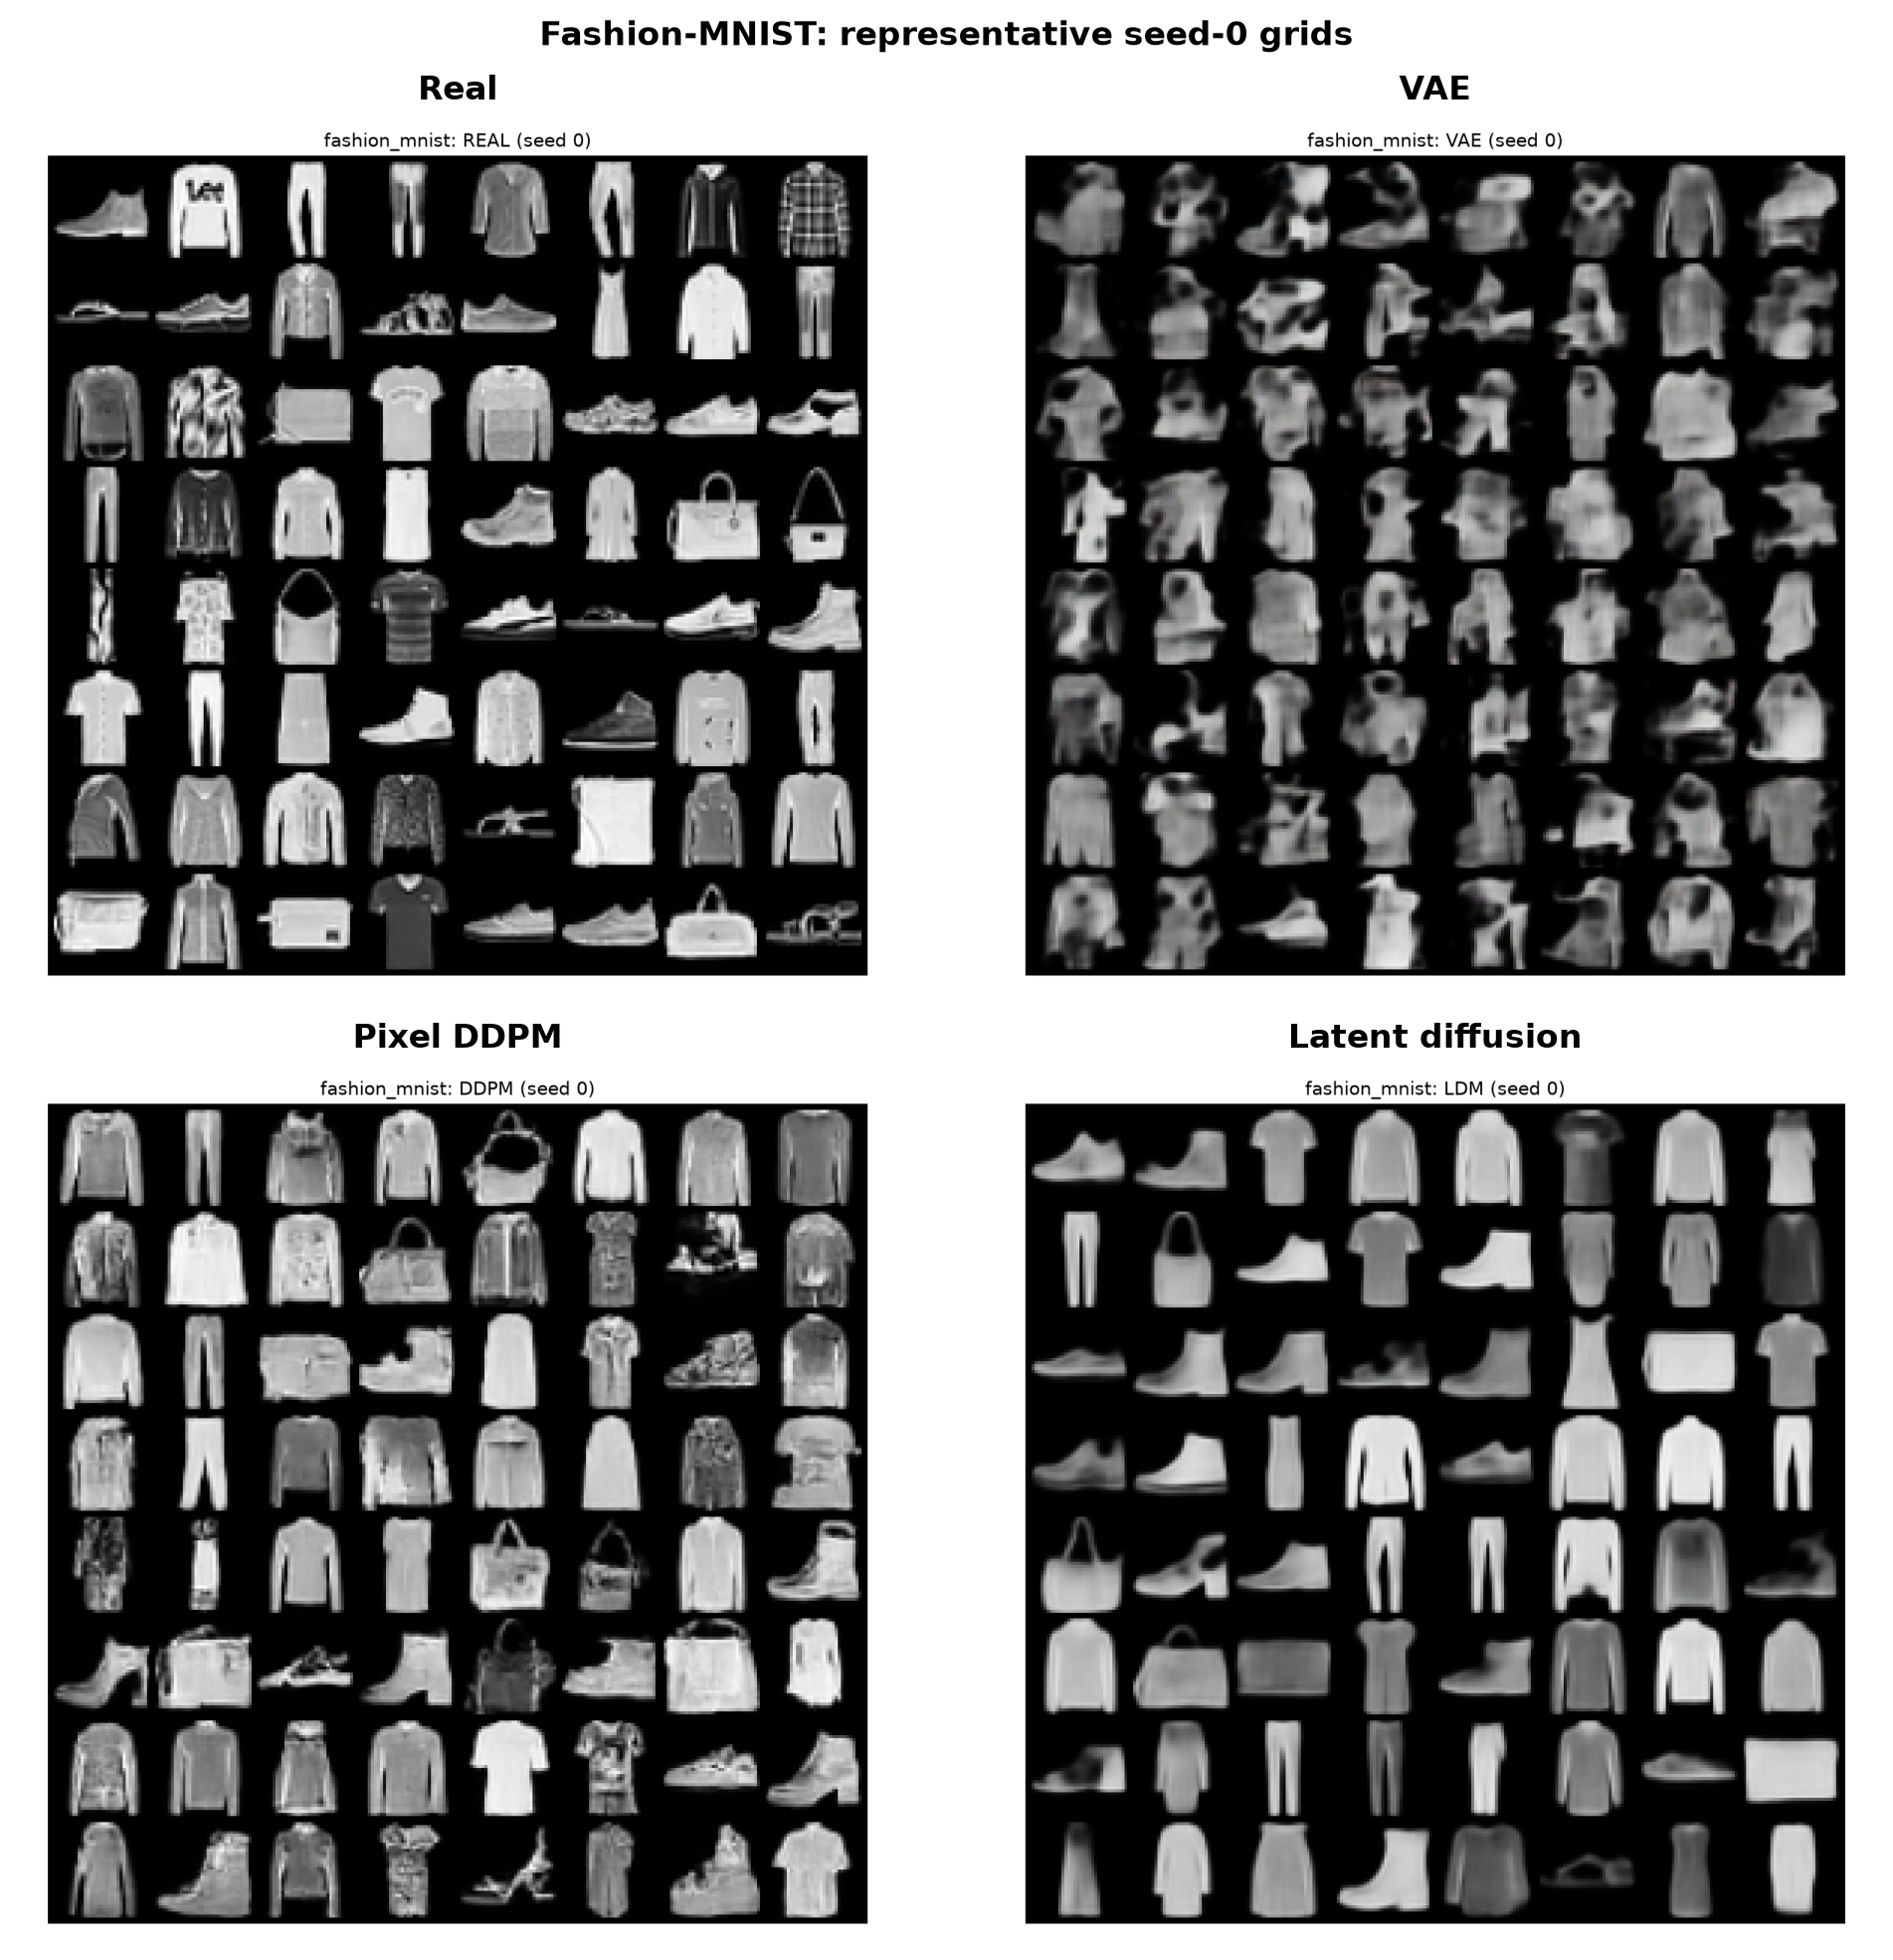
\includegraphics[width=\linewidth]{figures/qualitative_fashion_mnist.png}
  \small (a) Fashion-MNIST
\end{minipage}
\hfill
\begin{minipage}{0.47\linewidth}
  \centering
  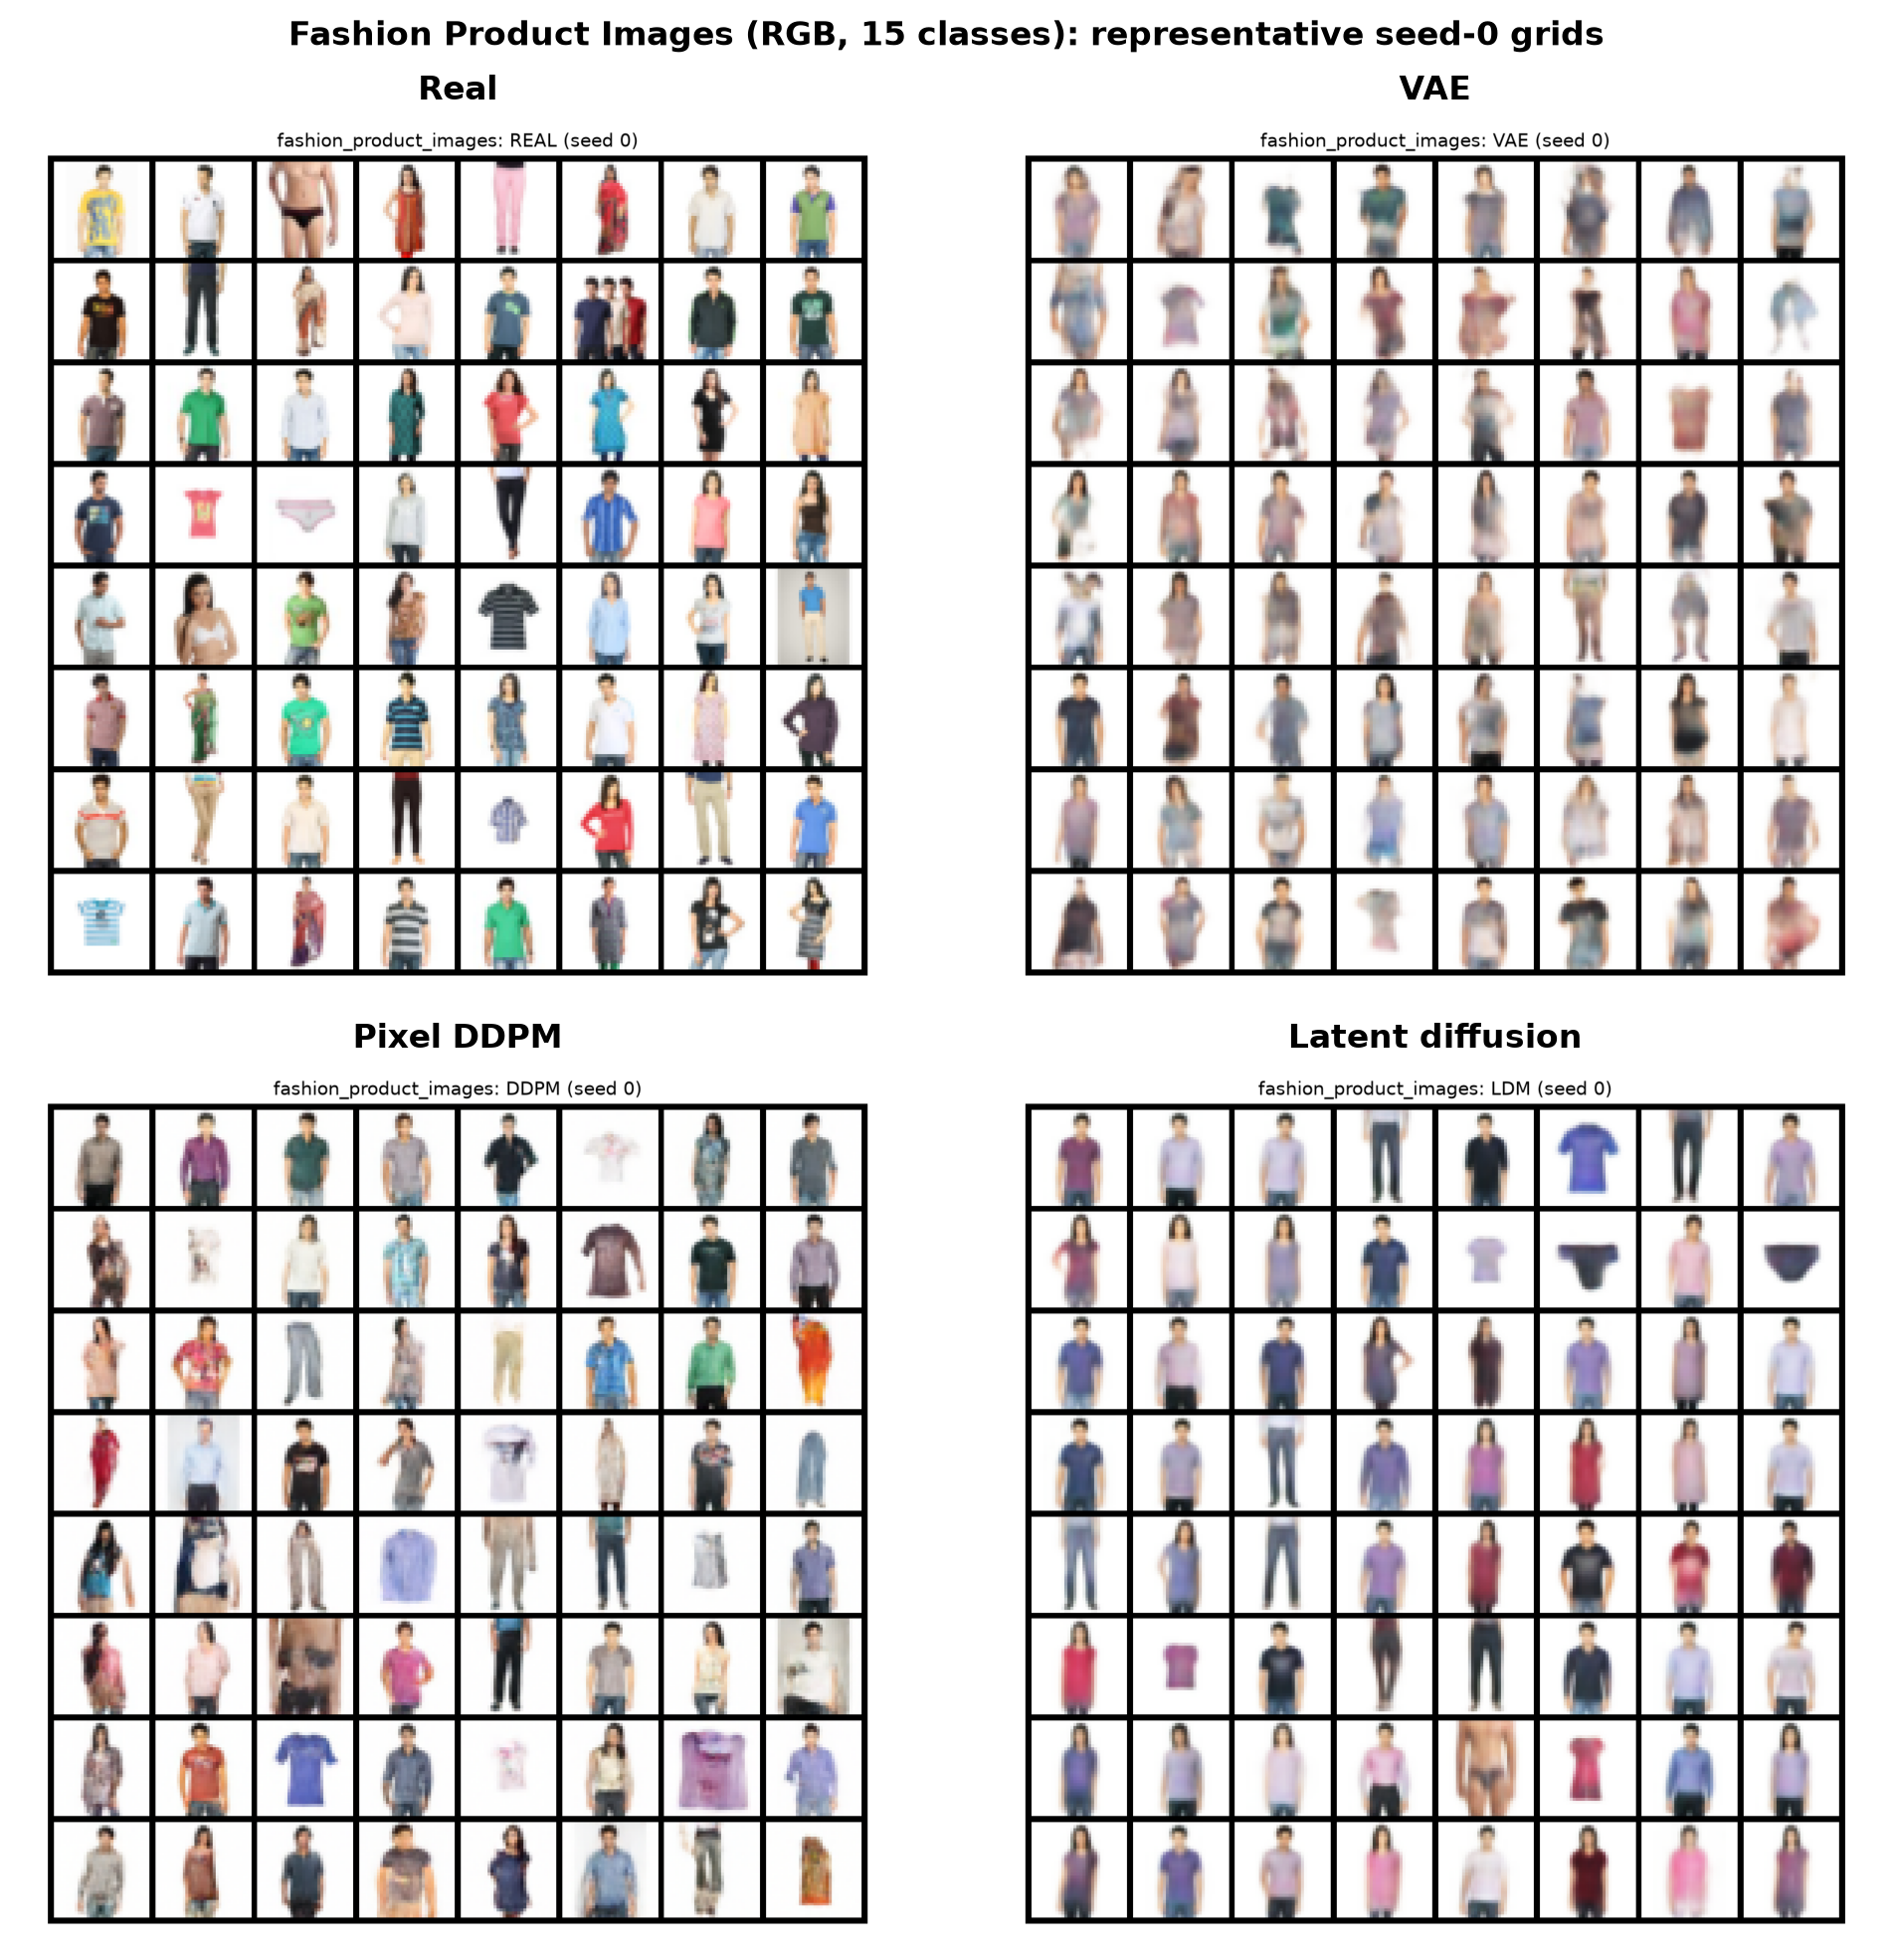
\includegraphics[width=\linewidth]{figures/qualitative_fashion_product_images.png}
  \small (b) Color products
\end{minipage}
\caption{Representative real and generated grids from seed 0.}
\label{fig:qualitative}
\end{figure}

Figure~\ref{fig:qualitative} and Table~\ref{tab:quality} show the same distribution-fidelity ordering on both datasets. DDPM reduces VAE FID by 75.1\% on Fashion-MNIST and 80.1\% on color products; it reduces LDM FID by 43.0\% and 50.5\%. KID corroborates rather than reverses this result: relative to VAE, DDPM lowers KID by 68.7\% and 77.9\%. Its JSD reductions are 80.2\% and 89.8\%, showing that its advantage extends from feature moments to class-proportion agreement.

The ordering is not caused by one favorable initialization. Fashion-MNIST FID ranges are 28.13--31.39 (DDPM), 50.79--52.60 (LDM), and 116.19--122.62 (VAE); the corresponding color ranges are 15.46--17.78, 32.25--37.54, and 79.21--89.73. Thus, the best and worst seed intervals in Figure~\ref{fig:seed-fid} do not overlap, and every model--dataset FID coefficient of variation is below 6.6\%. Absolute values must not be compared across datasets because each uses a different evaluator and the color test set has fewer real references.

\begin{table}[ht]
\caption{Generation quality, mean $\pm$ sample SD over five seeds. Lower FID, KID, and JSD are better; higher confidence and recognizability are better.}
\label{tab:quality}
\centering
\scriptsize
\begin{tabular}{llrrrrr}
\toprule
Dataset & Model & FID $\downarrow$ & KID $\downarrow$ & Confidence $\uparrow$ & Recog. $\uparrow$ & JSD $\downarrow$ \\
\midrule
Fashion-MNIST & VAE  & $119.10\pm2.87$ & $1.113\pm.021$ & $.794\pm.004$ & $.573\pm.010$ & $.077\pm.005$ \\
 & DDPM & $29.64\pm1.49$ & $.349\pm.019$ & $.928\pm.002$ & $.853\pm.007$ & $.015\pm.002$ \\
 & LDM  & $52.01\pm.71$ & $.687\pm.015$ & $.951\pm.002$ & $.899\pm.006$ & $.025\pm.002$ \\
\midrule
Color products & VAE  & $83.88\pm3.80$ & $.940\pm.049$ & $.790\pm.006$ & $.572\pm.012$ & $.061\pm.007$ \\
 & DDPM & $16.67\pm.85$ & $.208\pm.016$ & $.879\pm.003$ & $.756\pm.007$ & $.006\pm.001$ \\
 & LDM  & $33.65\pm2.21$ & $.429\pm.045$ & $.896\pm.007$ & $.790\pm.015$ & $.027\pm.003$ \\
\bottomrule
\end{tabular}
\end{table}

\begin{figure}[H]
\centering
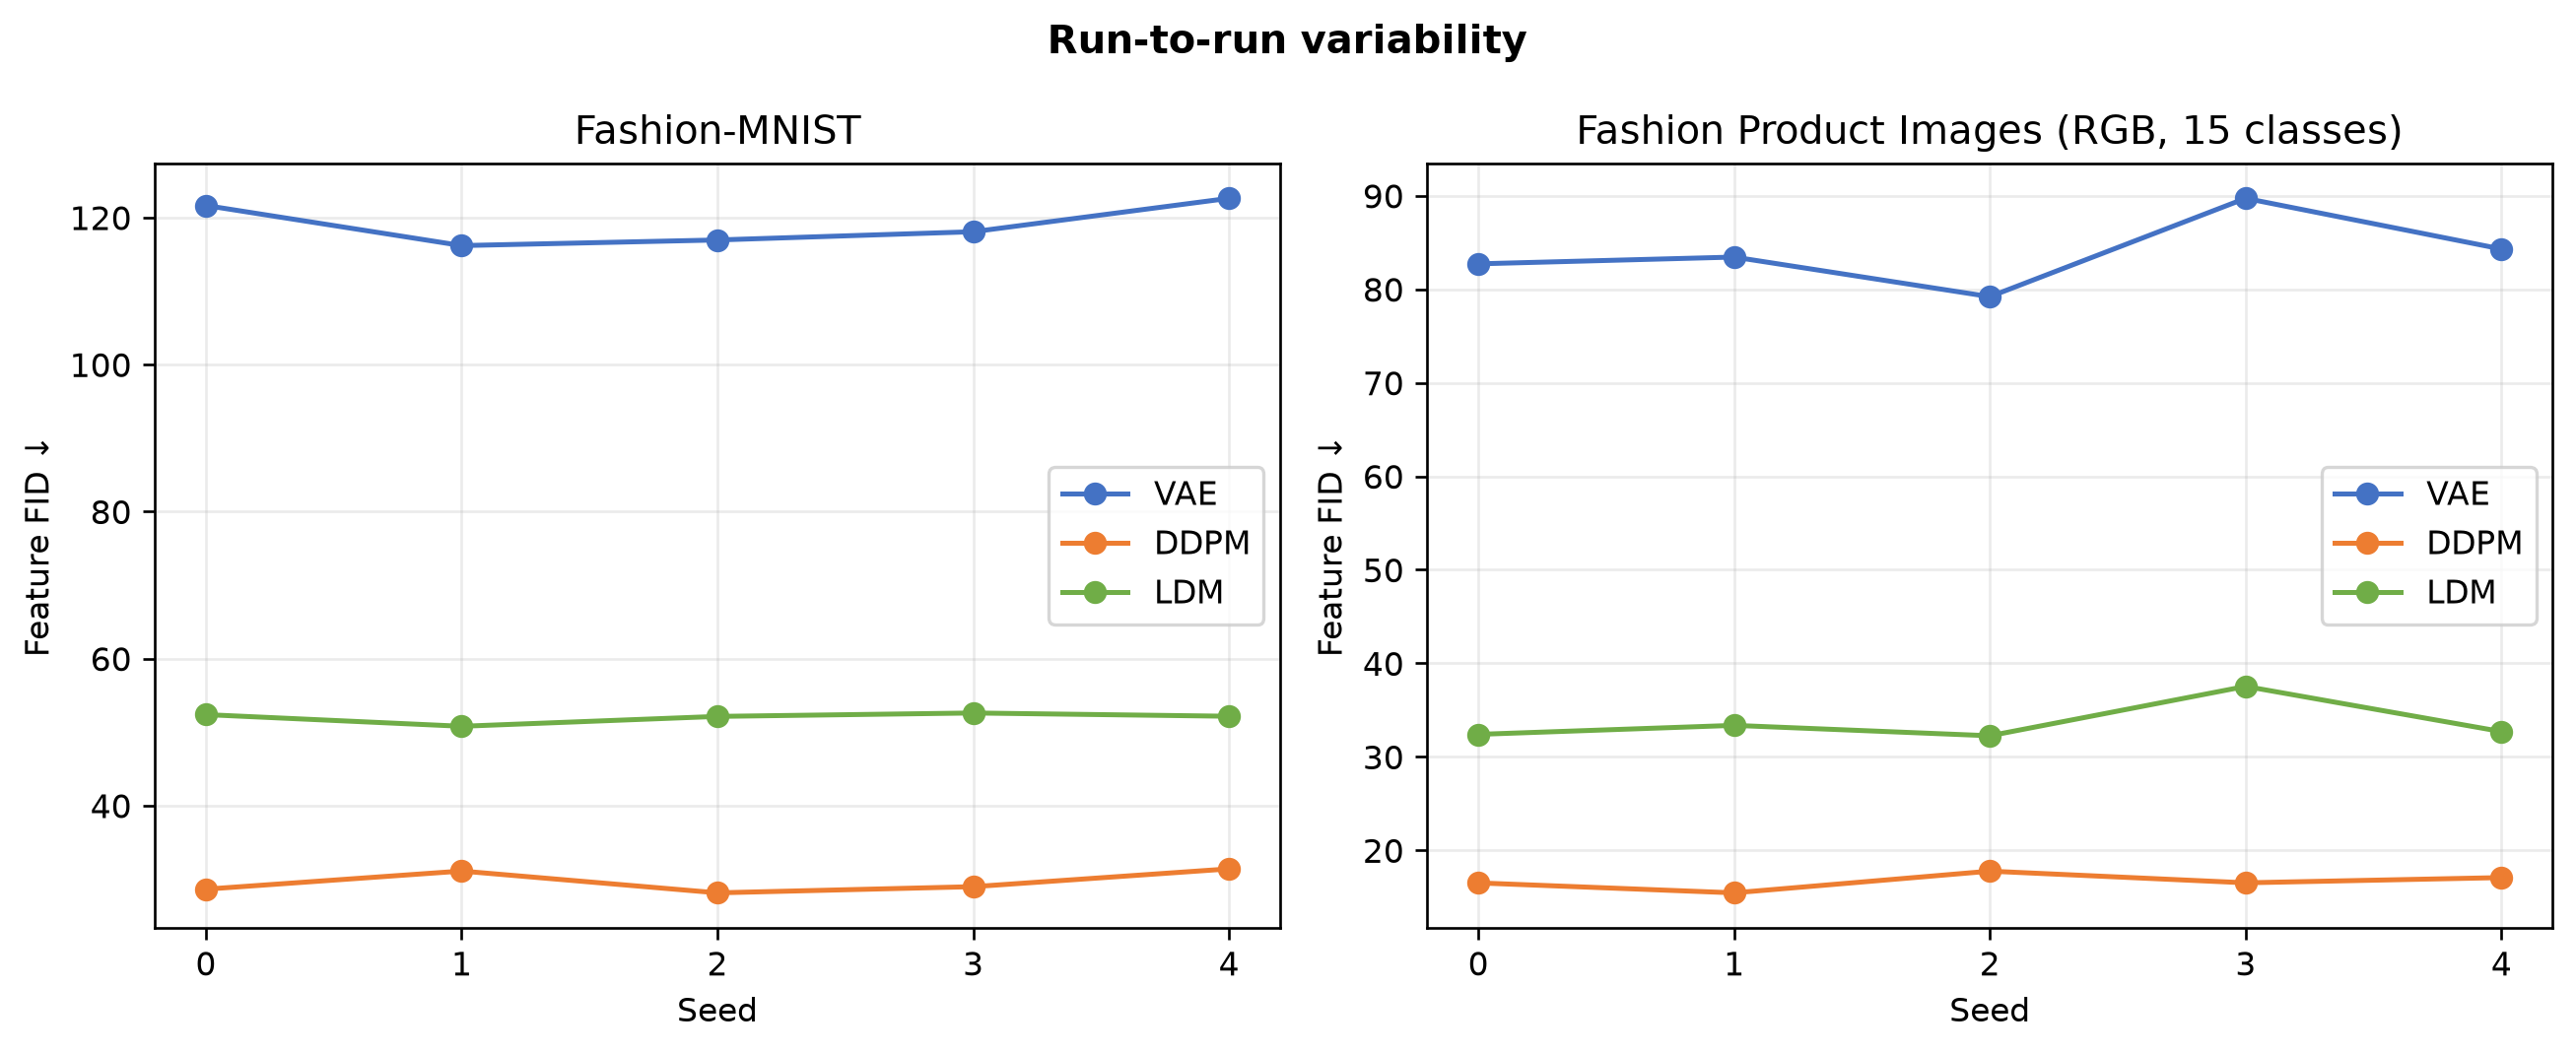
\includegraphics[width=0.78\linewidth]{figures/seed_variability.png}
\caption{Feature FID for every independently trained seed. Lines aid ranking comparison and do not imply a continuous seed variable.}
\label{fig:seed-fid}
\end{figure}

\subsection{Recognizability, diversity, and sharpness}
LDM has the highest confidence and recognizability: it exceeds DDPM recognizability by 4.62 percentage points on Fashion-MNIST and 3.46 points on color products. Its smoother, classifier-friendly images therefore look semantically decisive even though DDPM better matches the complete real distribution. All systems cover all 10 or 15 evaluator-predicted classes in every seed, so coverage alone fails to distinguish them.

\begin{table}[ht]
\caption{Supporting sample statistics, mean $\pm$ sample SD. cIS is classifier-based Inception Score; feature distance is the mean pairwise distance in evaluator space. Higher values are not unconditionally better.}
\label{tab:supporting}
\centering
\scriptsize
\begin{tabular}{llrrrr}
\toprule
Dataset & Model & Entropy & cIS & Feature distance & Sobel sharpness \\
\midrule
Fashion-MNIST & VAE  & $.868\pm.008$ & $4.293\pm.100$ & $13.005\pm.143$ & $.546\pm.008$ \\
 & DDPM & $.973\pm.004$ & $7.785\pm.088$ & $19.595\pm.042$ & $.608\pm.009$ \\
 & LDM  & $.960\pm.003$ & $8.079\pm.049$ & $20.480\pm.112$ & $.507\pm.011$ \\
\midrule
Color products & VAE  & $.644\pm.019$ & $3.405\pm.104$ & $13.812\pm.131$ & $.767\pm.003$ \\
 & DDPM & $.728\pm.010$ & $5.283\pm.091$ & $18.356\pm.103$ & $.827\pm.002$ \\
 & LDM  & $.734\pm.008$ & $5.637\pm.070$ & $18.984\pm.181$ & $.782\pm.002$ \\
\bottomrule
\end{tabular}
\end{table}

Table~\ref{tab:supporting} explains the metric disagreement. LDM leads cIS and pairwise feature distance on both datasets, consistent with confident, well-separated semantic samples, but DDPM leads FID, KID, and JSD. On the imbalanced color set, LDM has slightly higher normalized entropy than DDPM ($.734$ versus $.728$) yet over four times its JSD ($.0268$ versus $.0062$): uniformity is not the target when the real distribution is nonuniform. DDPM also has the highest Sobel magnitude on both datasets. The low Fashion-MNIST LDM value ($.507$) supports visible decoder smoothing, whereas the higher color-domain values partly reflect photographic edges and backgrounds rather than garment fidelity. Five-seed class distributions are shown in Appendix~\ref{app:diagnostics}.

\subsection{Efficiency and stability}

Across datasets, VAE requires 1.61--1.66 minutes to train and 0.036 ms/image to sample; LDM requires 3.48--3.78 minutes and 0.763--0.765 ms/image; DDPM requires 5.55--5.62 minutes and 10.611--10.624 ms/image. LDM is 13.9 times faster than DDPM and reduces its end-to-end training time by 33--37\%; VAE is about 292 times faster than DDPM and 21 times faster than LDM. These batched rates correspond approximately to 27,600, 1,310, and 94 images/s for VAE, LDM, and DDPM, not single-request latency.

Complete-system parameter counts are 1.955M, 7.743M, and 5.787M for VAE, LDM, and DDPM. Despite having 33.8\% more parameters than DDPM because its total includes the autoencoder, LDM has 32\% lower measured peak memory: 5.20--5.21 GB versus 7.68--7.70 GB. VAE peaks at 6.30--6.32 GB. This inversion shows that the 4,096-sample activation geometry, rather than weights alone, dominates high-throughput inference memory. All 30 runs have finite losses and no detected collapse. Appendix~\ref{app:diagnostics} provides convergence and separate training/sampling memory plots.

\begin{table}[H]
\caption{Computational results, mean $\pm$ sample SD over five seeds. LDM totals include its VAE; sampling is batched throughput.}
\label{tab:compute}
\centering
\scriptsize
\resizebox{\linewidth}{!}{\begin{tabular}{llrrrr}
\toprule
Dataset & Model & Train (min) $\downarrow$ & Batched sample (ms/image) $\downarrow$ & Parameters (M) $\downarrow$ & Peak GPU (MB) $\downarrow$ \\
\midrule
Fashion-MNIST & VAE & 1.61 $\pm$ 0.00 & 0.036 $\pm$ 0.000 & 1.955 $\pm$ 0.000 & 6301 $\pm$ 4 \\
 & DDPM & 5.55 $\pm$ 0.00 & 10.611 $\pm$ 0.008 & 5.787 $\pm$ 0.000 & 7683 $\pm$ 0 \\
 & LDM & 3.48 $\pm$ 0.05 & 0.763 $\pm$ 0.001 & 7.743 $\pm$ 0.000 & 5196 $\pm$ 0 \\
\midrule
Fashion Product Images (RGB, 15 classes) & VAE & 1.66 $\pm$ 0.00 & 0.036 $\pm$ 0.000 & 1.955 $\pm$ 0.000 & 6318 $\pm$ 0 \\
 & DDPM & 5.62 $\pm$ 0.01 & 10.624 $\pm$ 0.011 & 5.787 $\pm$ 0.000 & 7698 $\pm$ 0 \\
 & LDM & 3.78 $\pm$ 0.01 & 0.765 $\pm$ 0.003 & 7.743 $\pm$ 0.000 & 5211 $\pm$ 0 \\
\bottomrule
\end{tabular}}
\end{table}

\section{Discussion}
\subsection{Model-selection implications}
DDPM is preferred when distribution fidelity and class-proportion agreement dominate: it leads FID, KID, and JSD in every seed. LDM is the best compromise when pixel diffusion is too expensive; it accepts 43--50\% higher FID than DDPM but removes 92.8\% of diffusion sampling time and leads recognizability and cIS. This disagreement shows that individually clear samples can still misrepresent global feature and class statistics. VAE is appropriate when speed and model size dominate, at a substantial fidelity cost. Because optimizer settings were selected on Fashion-MNIST and transferred unchanged, the persistent color-domain ranking demonstrates robustness without test-set tuning, not color-domain optimality.

\subsection{Robustness and limitations}
The systems are neither parameter- nor FLOP-matched, so conclusions concern complete implementations rather than objectives in isolation. Fixed updates also expose the 8,007-image color set more often than Fashion-MNIST. Its 1,423-reference test set and imperfect evaluator add uncertainty, while FID, KID, cIS, confidence, and feature distance reuse the same features; cross-dataset values are therefore not comparable. Timings measure RTX 5070 Ti throughput at large batch size, not interactive latency. Finally, the common 100-step ancestral sampler controls reverse depth but may miss each diffusion model's best frontier. Priority follow-ups are equal-compute comparisons, independent feature spaces, real-reference bootstrapping, and step-count/solver ablations.

\section{Conclusions}
Across both apparel domains, pixel DDPM gives the closest distribution, LDM the best quality--throughput compromise, and VAE the greatest speed and compactness. The stable five-seed ranking defines a use-dependent frontier; recognizability and feature fidelity can diverge. Future work should match compute, test faster samplers, strengthen the latent objective, and use independent features.

\clearpage
\begin{thebibliography}{99}
\bibitem{kingma2014vae} D. P. Kingma and M. Welling, ``Auto-Encoding Variational Bayes,'' in \emph{Proc. 2nd Int. Conf. Learning Representations (ICLR)}, 2014. [Online]. Available: \url{https://arxiv.org/abs/1312.6114}

\bibitem{ho2020ddpm} J. Ho, A. Jain, and P. Abbeel, ``Denoising Diffusion Probabilistic Models,'' in \emph{Advances in Neural Information Processing Systems}, vol. 33, pp. 6840--6851, 2020. [Online]. Available: \url{https://arxiv.org/abs/2006.11239}

\bibitem{rombach2022ldm} R. Rombach, A. Blattmann, D. Lorenz, P. Esser, and B. Ommer, ``High-Resolution Image Synthesis with Latent Diffusion Models,'' in \emph{Proc. IEEE/CVF Conf. Computer Vision and Pattern Recognition (CVPR)}, pp. 10684--10695, 2022. [Online]. Available: \url{https://arxiv.org/abs/2112.10752}

\bibitem{nichol2021improved} A. Q. Nichol and P. Dhariwal, ``Improved Denoising Diffusion Probabilistic Models,'' in \emph{Proc. 38th Int. Conf. Machine Learning (ICML)}, pp. 8162--8171, 2021. [Online]. Available: \url{https://arxiv.org/abs/2102.09672}

\bibitem{xiao2017fashion} H. Xiao, K. Rasul, and R. Vollgraf, ``Fashion-MNIST: A Novel Image Dataset for Benchmarking Machine Learning Algorithms,'' 2017. [Online]. Available: \url{https://arxiv.org/abs/1708.07747}

\bibitem{fpis} Transformersx, ``Fashion Product Images Small,'' Hugging Face Datasets. [Online]. Available: \url{https://huggingface.co/datasets/Transformersx/fashion-product-images-small}. Accessed: Aug. 12, 2026.

\bibitem{he2016resnet} K. He, X. Zhang, S. Ren, and J. Sun, ``Deep Residual Learning for Image Recognition,'' in \emph{Proc. IEEE Conf. Computer Vision and Pattern Recognition (CVPR)}, pp. 770--778, 2016. [Online]. Available: \url{https://arxiv.org/abs/1512.03385}

\bibitem{loshchilov2019adamw} I. Loshchilov and F. Hutter, ``Decoupled Weight Decay Regularization,'' in \emph{Proc. 7th Int. Conf. Learning Representations (ICLR)}, 2019. [Online]. Available: \url{https://arxiv.org/abs/1711.05101}

\bibitem{heusel2017fid} M. Heusel, H. Ramsauer, T. Unterthiner, B. Nessler, and S. Hochreiter, ``GANs Trained by a Two Time-Scale Update Rule Converge to a Local Nash Equilibrium,'' in \emph{Advances in Neural Information Processing Systems}, vol. 30, 2017. [Online]. Available: \url{https://arxiv.org/abs/1706.08500}

\bibitem{binkowski2018kid} M. Bi\'nkowski, D. J. Sutherland, M. Arbel, and A. Gretton, ``Demystifying MMD GANs,'' in \emph{Proc. 6th Int. Conf. Learning Representations (ICLR)}, 2018. [Online]. Available: \url{https://arxiv.org/abs/1801.01401}

\bibitem{cui2019classbalanced} Y. Cui, M. Jia, T.-Y. Lin, Y. Song, and S. Belongie, ``Class-Balanced Loss Based on Effective Number of Samples,'' in \emph{Proc. IEEE/CVF Conf. Computer Vision and Pattern Recognition (CVPR)}, pp. 9268--9277, 2019. [Online]. Available: \url{https://arxiv.org/abs/1901.05555}
\end{thebibliography}

\clearpage
\appendix
\section*{Appendix}

\section{Hyperparameter Selection Evidence}
\label{app:tuning}
The classifier search compares batch size, training duration, learning rate, weight decay, and square-root inverse-frequency weighting motivated by class-balanced learning \citep{cui2019classbalanced}. The selected Fashion-MNIST evaluator uses learning rate $3\times10^{-4}$; the color evaluator uses $10^{-3}$. The unweighted color candidate wins the predefined mean accuracy/balanced-accuracy score, although weighting raises minimum validation recall from 25.00\% to 41.67\%. This trade-off motivates disclosure of balanced accuracy and per-class recall.

\begin{figure}[ht]
\centering
\begin{minipage}{0.49\linewidth}
  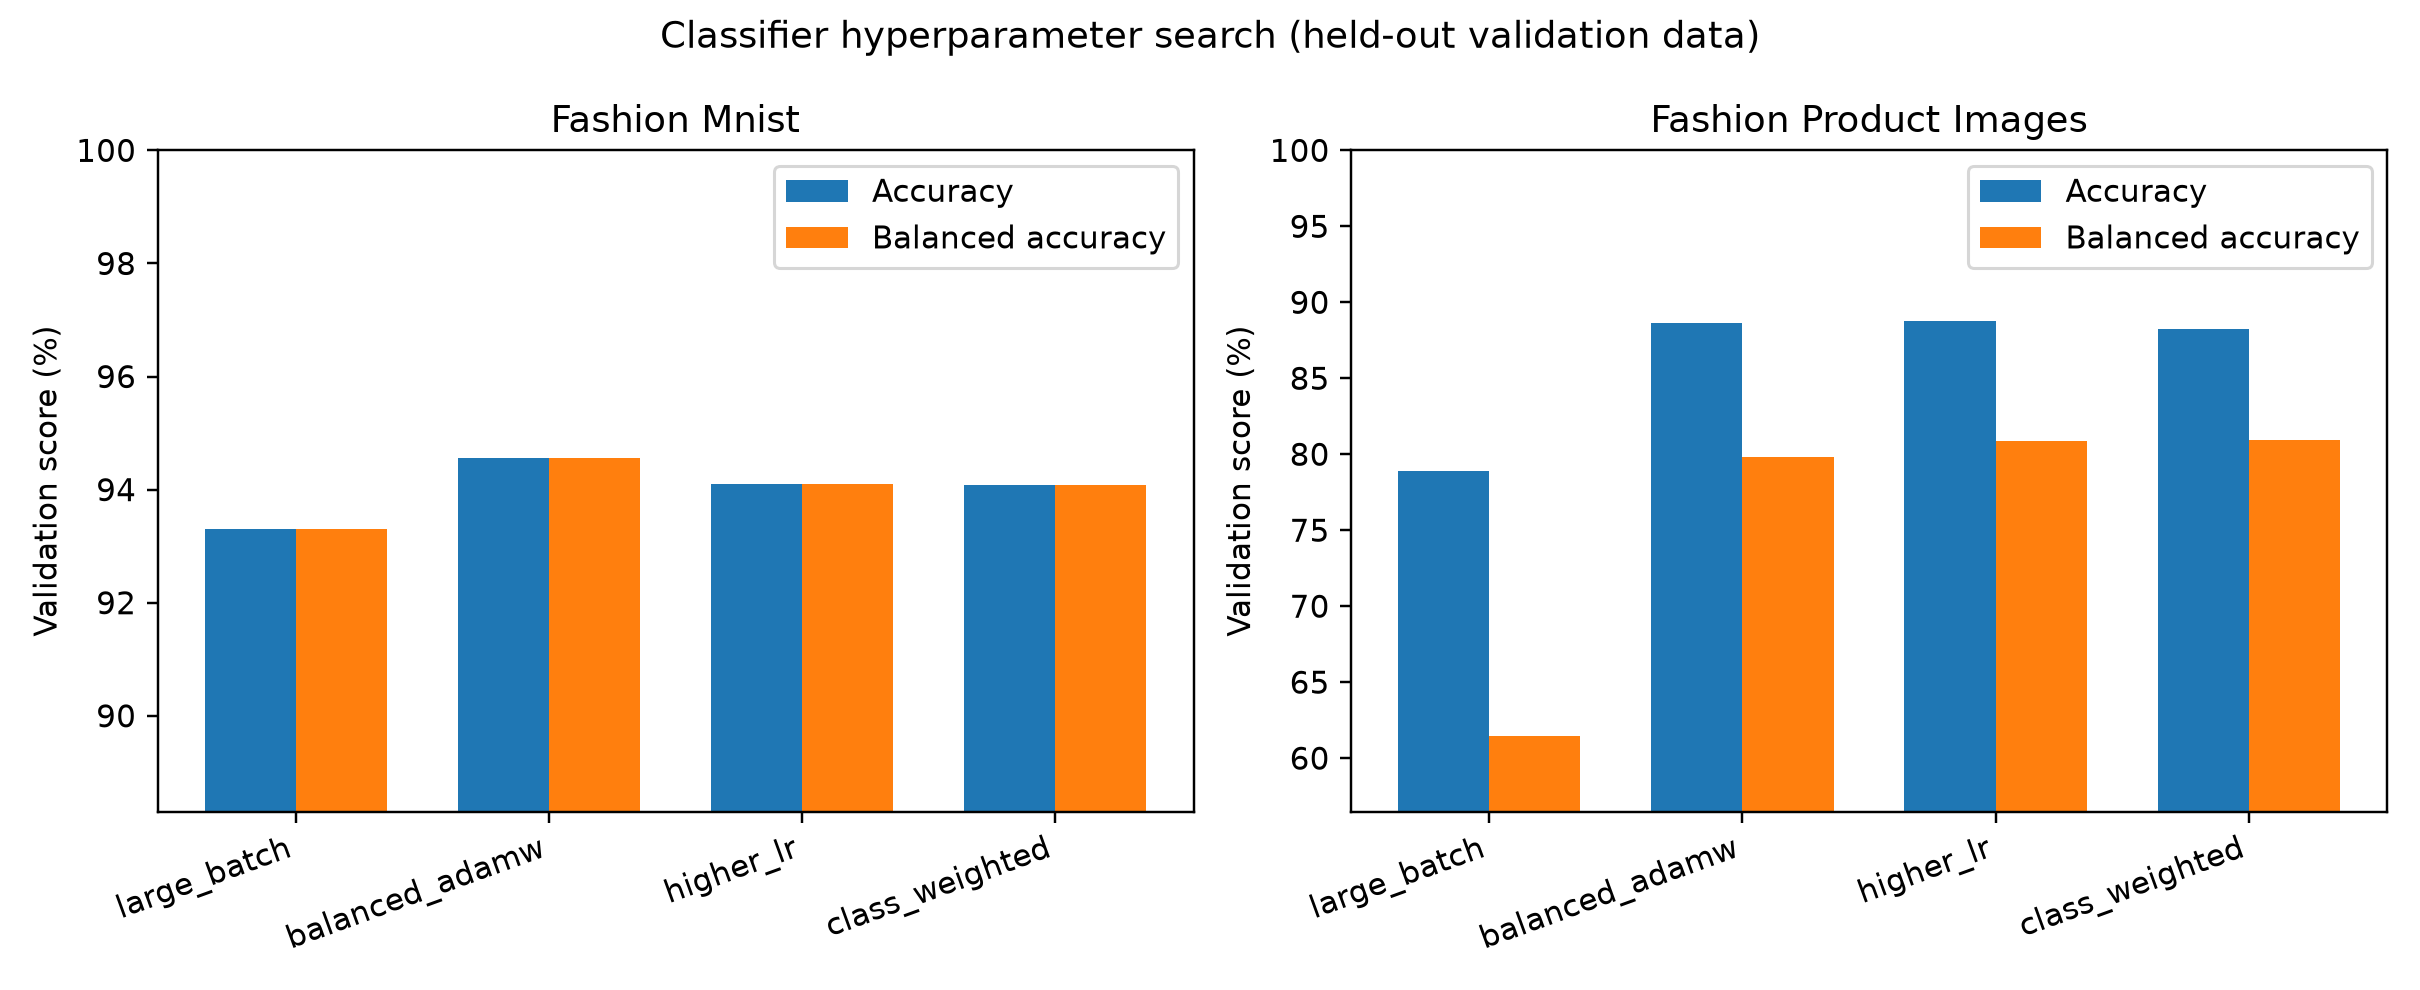
\includegraphics[width=\linewidth]{figures/classifier_hyperparameter_search.png}
  \small (a) Classifier search
\end{minipage}
\hfill
\begin{minipage}{0.49\linewidth}
  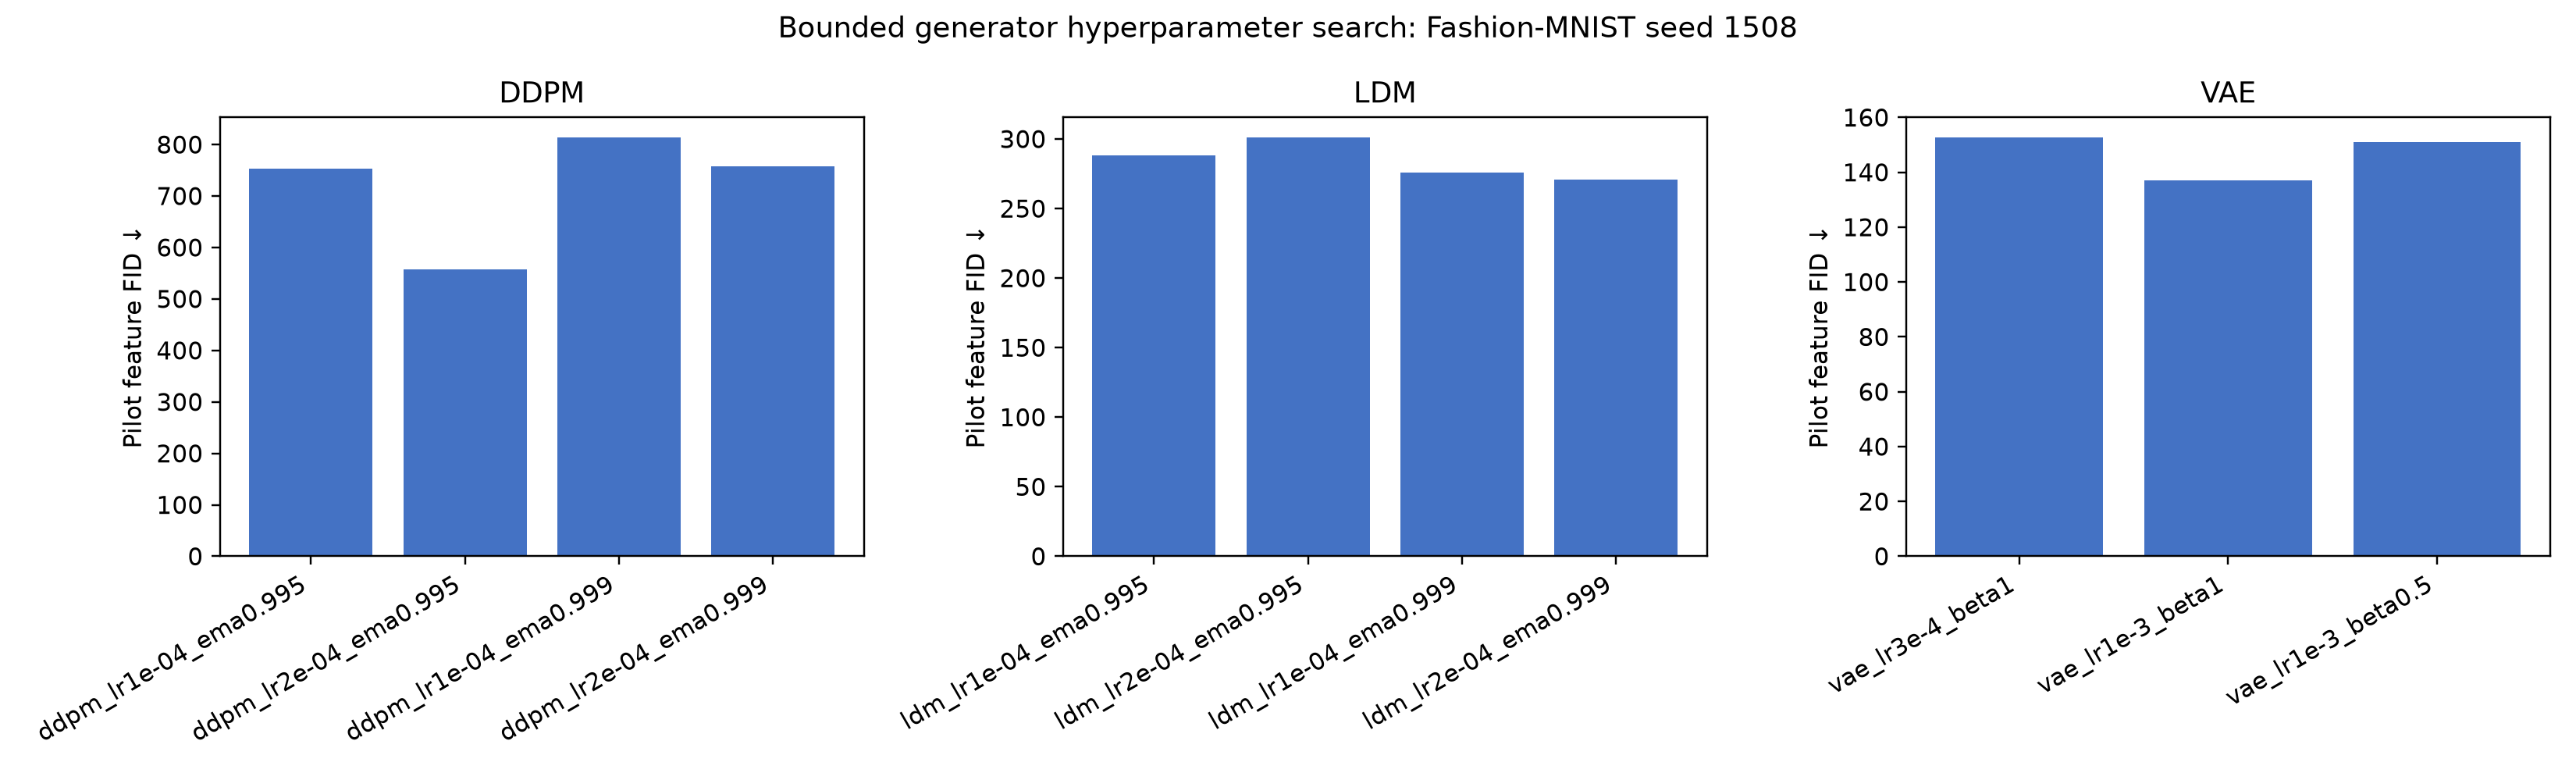
\includegraphics[width=\linewidth]{figures/generator_hyperparameter_search.png}
  \small (b) Generator pilot
\end{minipage}
\caption{Validation-only hyperparameter evidence. Short generator pilots select settings within each family and are not final quality results.}
\end{figure}

An initially unstable LDM produced standardized sampled latent SD 13.3 and maximum magnitude 327.3. Base width 64, exact posterior variance, and predicted-clean latent clipping at $\pm3$ reduce validation FID from 174.2 to 58.8 and sampled latent SD to 0.842. Pixel DDPM is tuned independently: exact-posterior sampling plus predicted-clean image clipping reduces validation FID from 68.86 to 34.04.

\begin{figure}[ht]
\centering
\begin{minipage}{0.32\linewidth}
  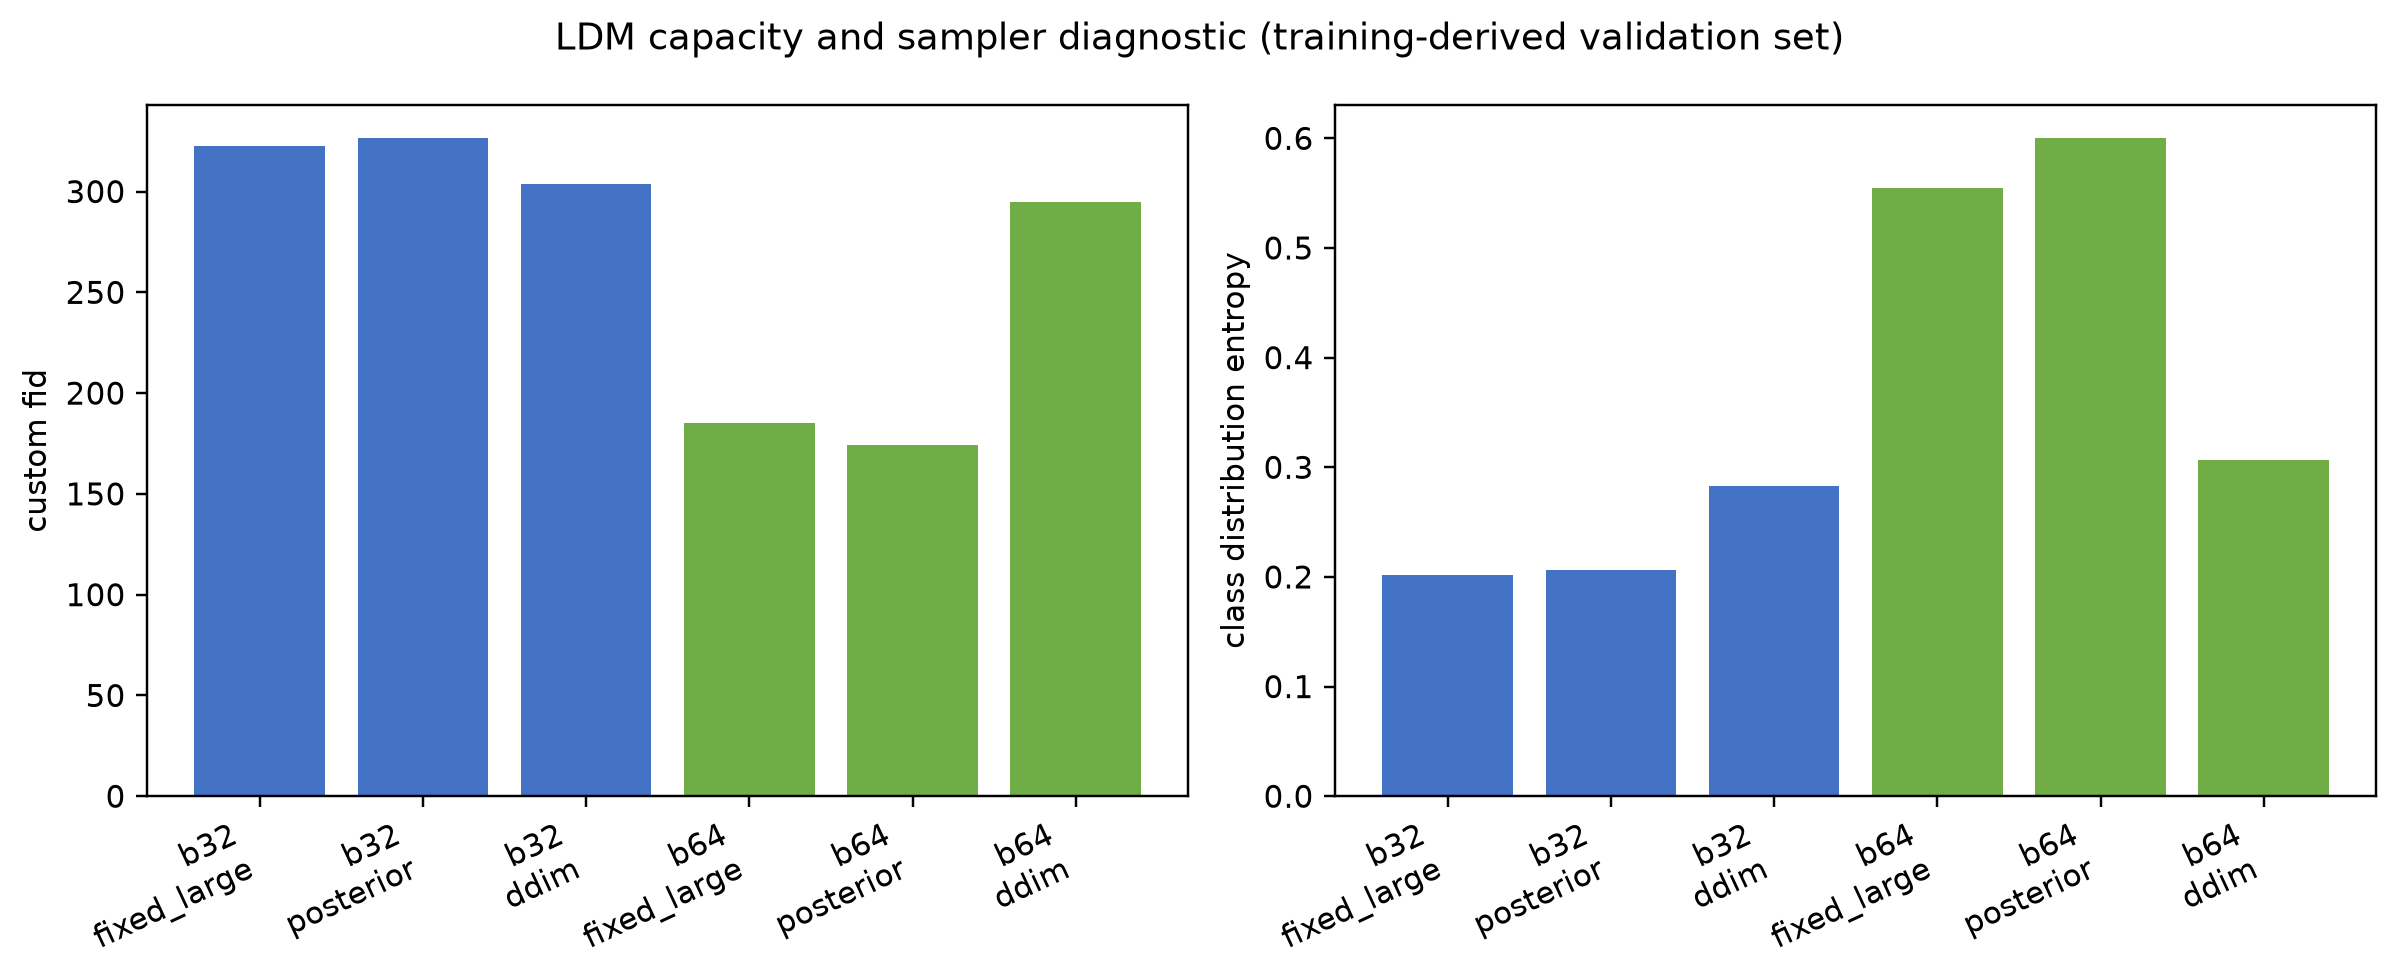
\includegraphics[width=\linewidth]{figures/ldm_capacity_sampler_diagnostic.png}
  \small (a) LDM width/sampler
\end{minipage}\hfill
\begin{minipage}{0.32\linewidth}
  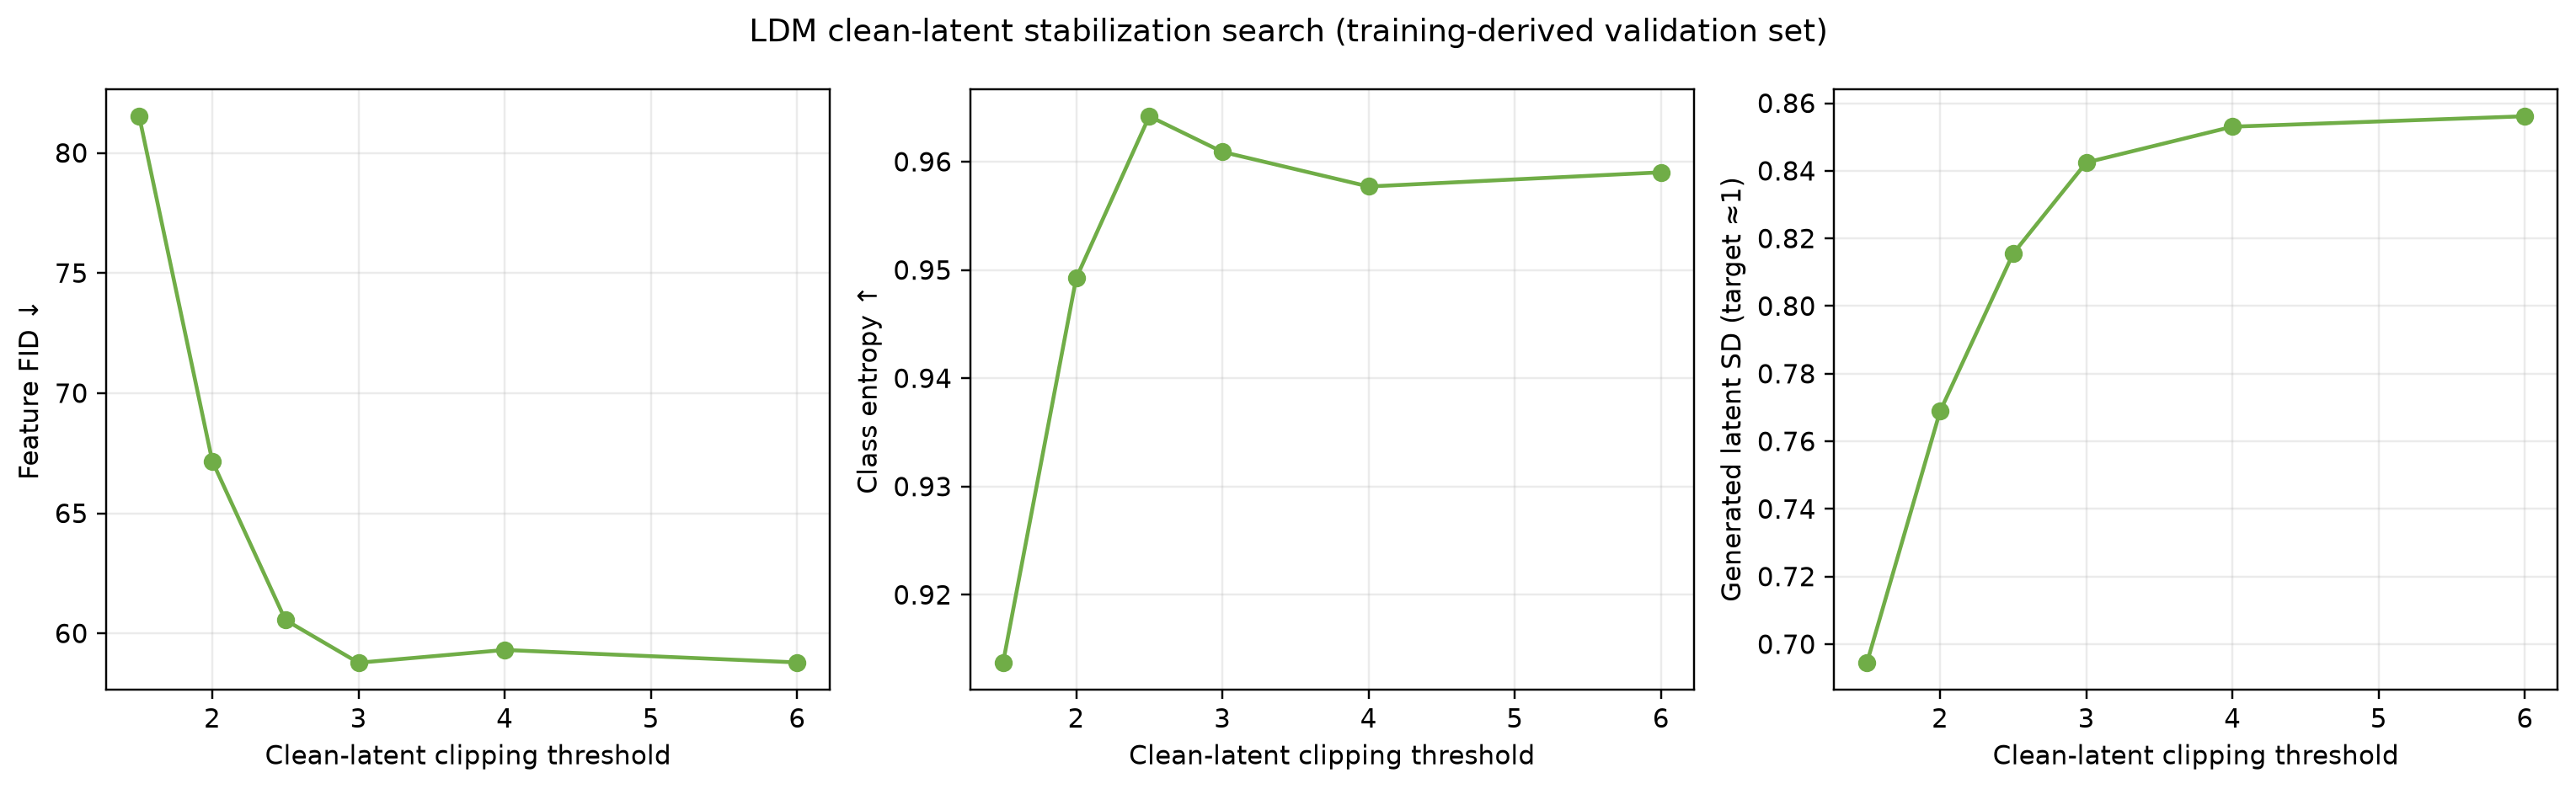
\includegraphics[width=\linewidth]{figures/ldm_clipping_search.png}
  \small (b) Latent clipping
\end{minipage}\hfill
\begin{minipage}{0.32\linewidth}
  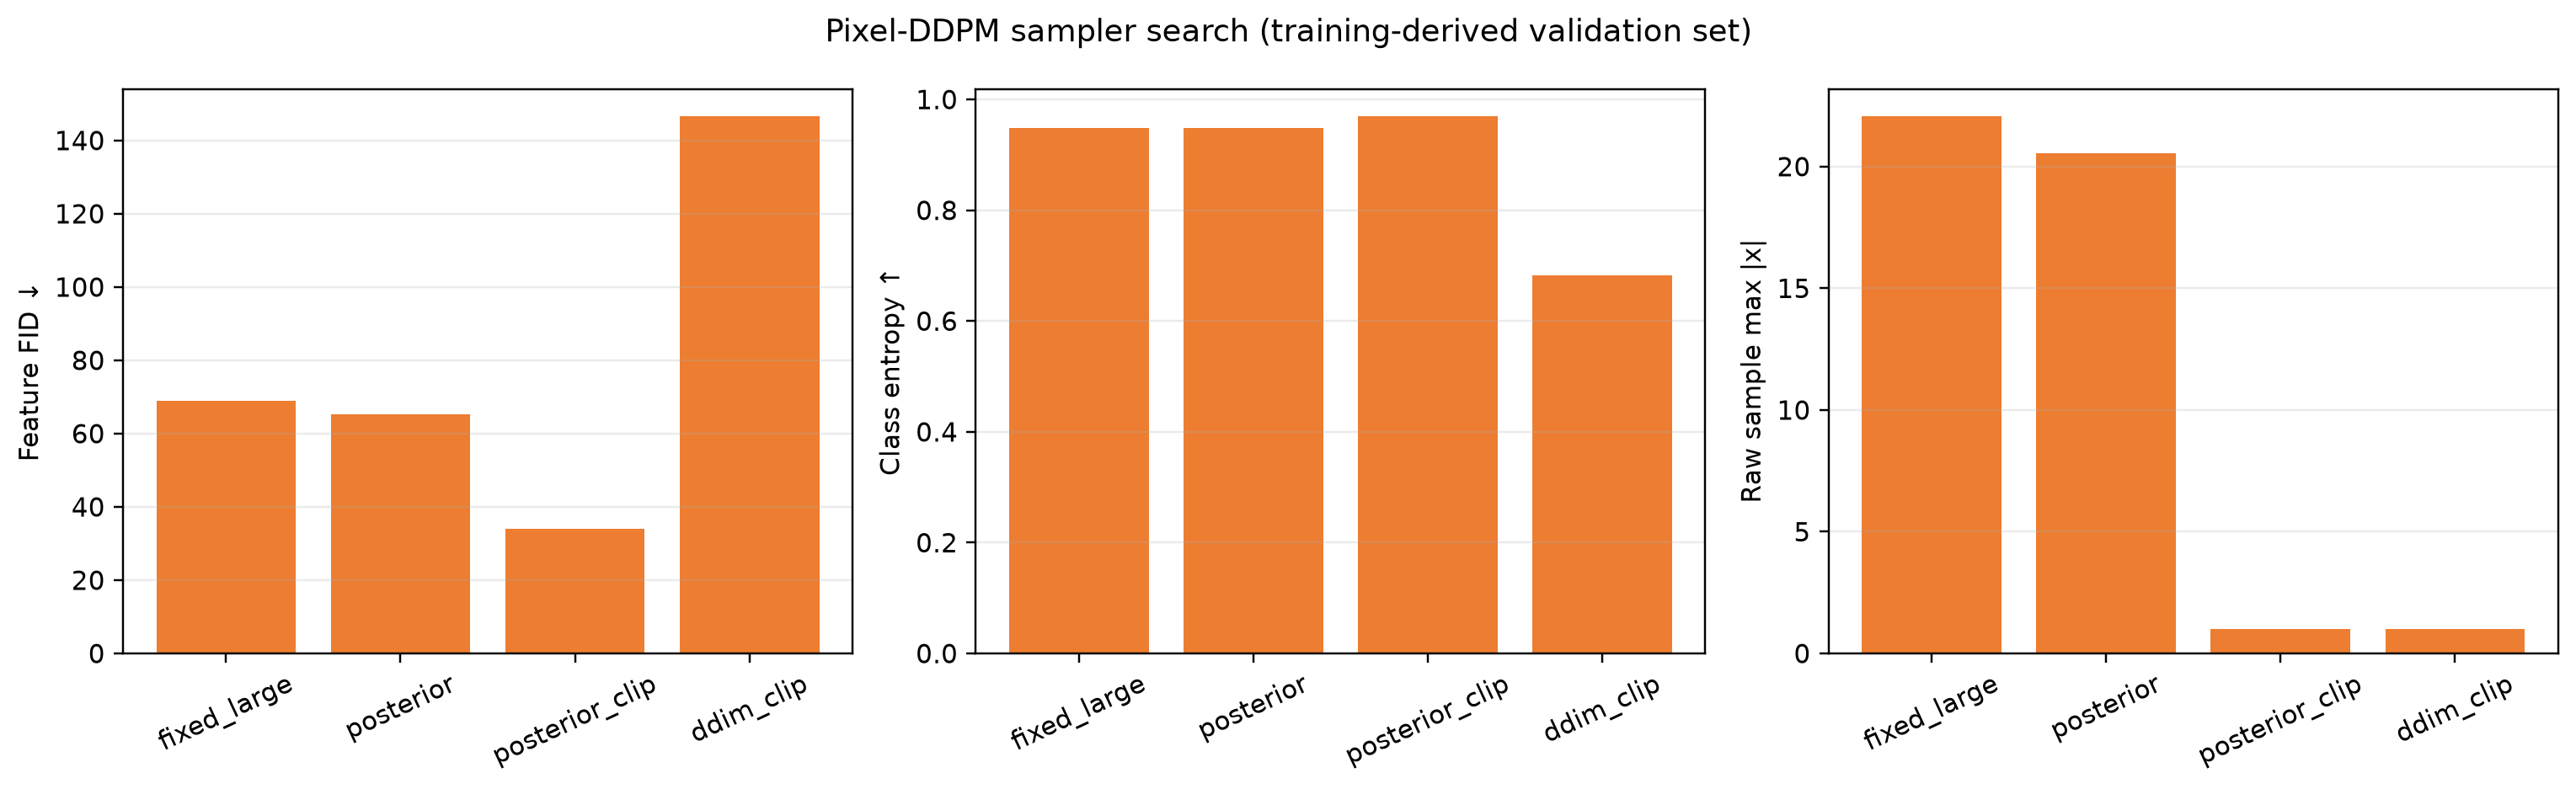
\includegraphics[width=\linewidth]{figures/ddpm_sampler_search.png}
  \small (c) DDPM sampler
\end{minipage}
\caption{Validation-only diffusion stabilization diagnostics.}
\end{figure}

\clearpage
\section{Evaluator and Dataset Diagnostics}
\label{app:evaluator}
\begin{figure}[ht]
  \centering
  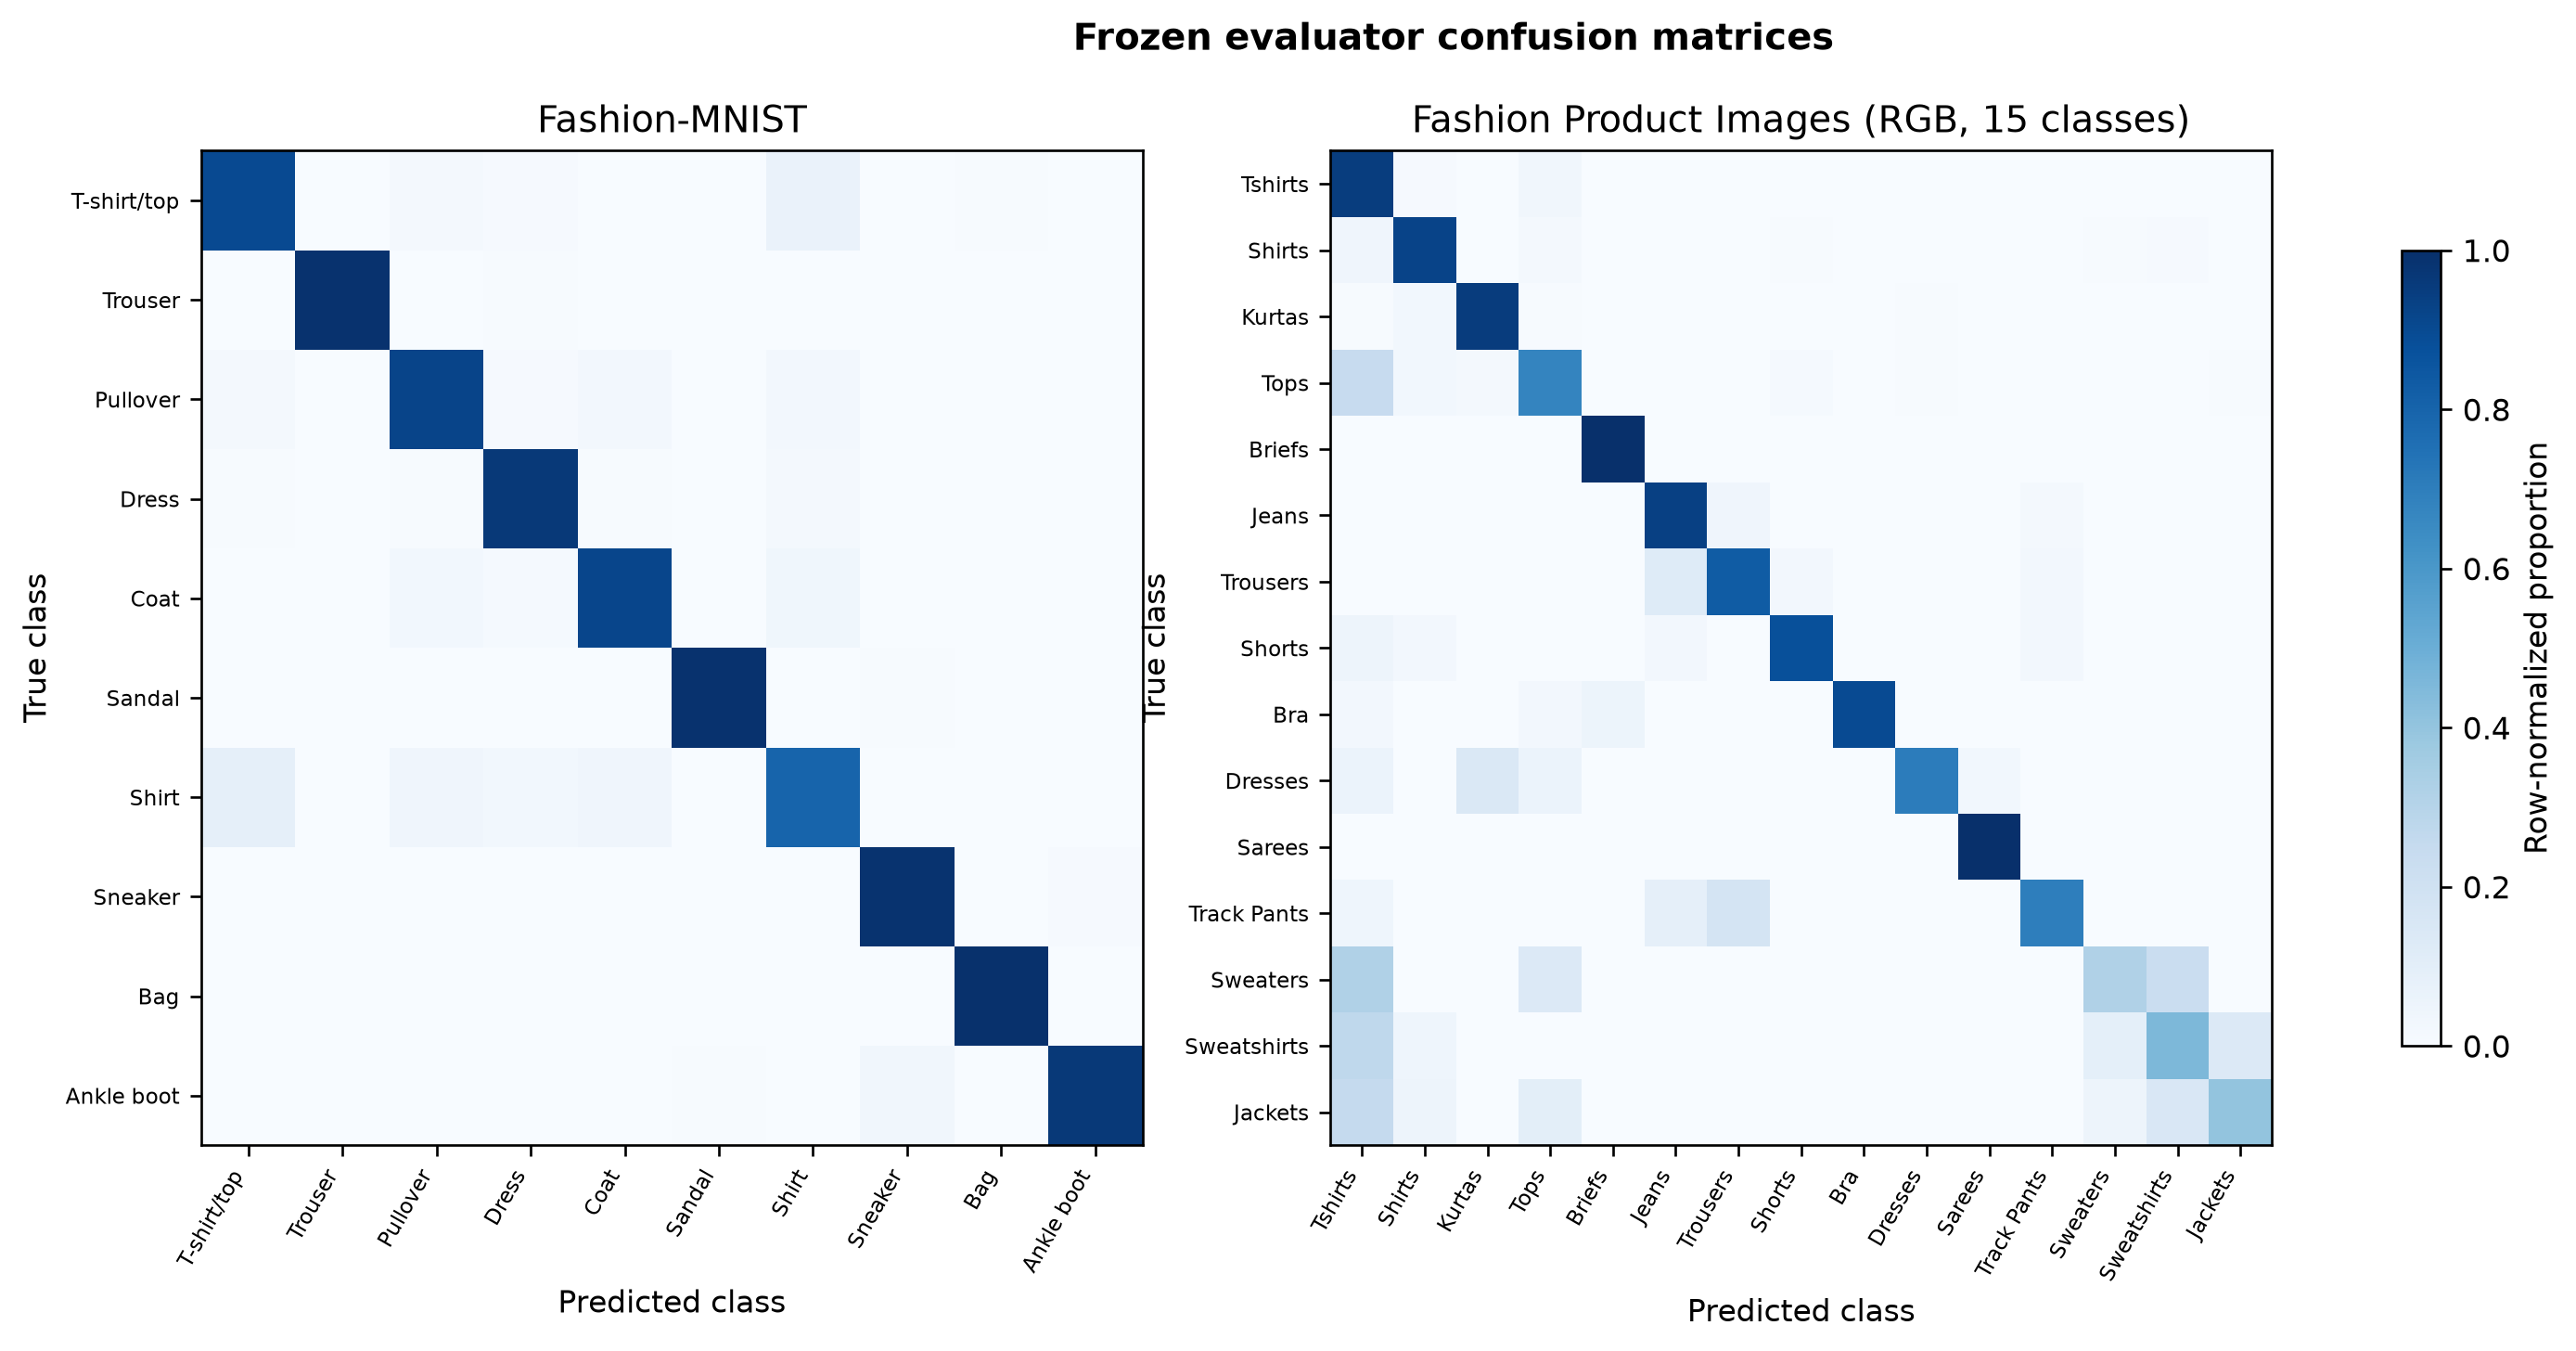
\includegraphics[width=0.95\linewidth]{figures/classifier_confusion_matrices.png}
  \caption{Row-normalized evaluator confusion matrices. Generator feature and class metrics inherit these errors.}
\end{figure}

\begin{figure}[ht]
\centering
\begin{minipage}{0.49\linewidth}
  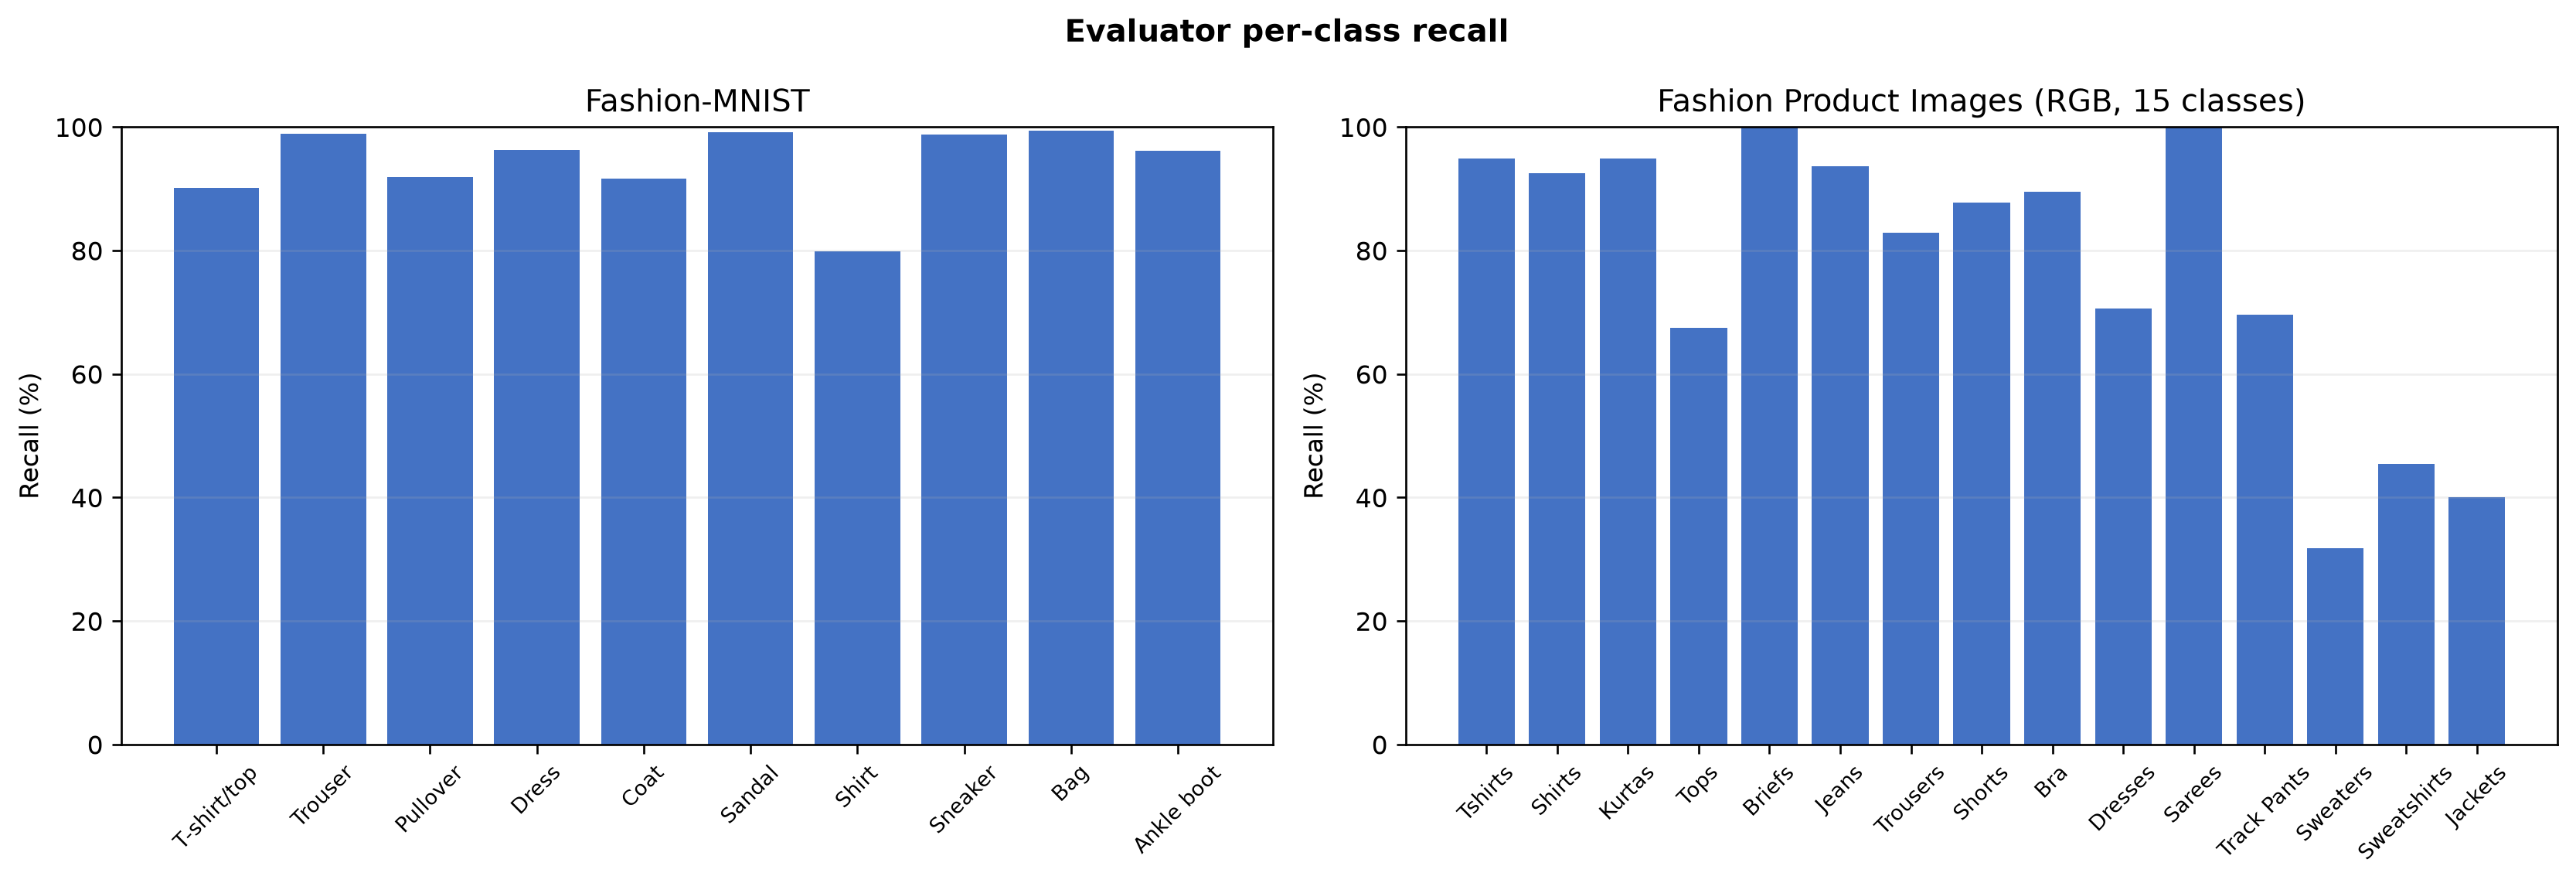
\includegraphics[width=\linewidth]{figures/classifier_per_class_recall.png}
  \small (a) Per-class recall
\end{minipage}\hfill
\begin{minipage}{0.49\linewidth}
  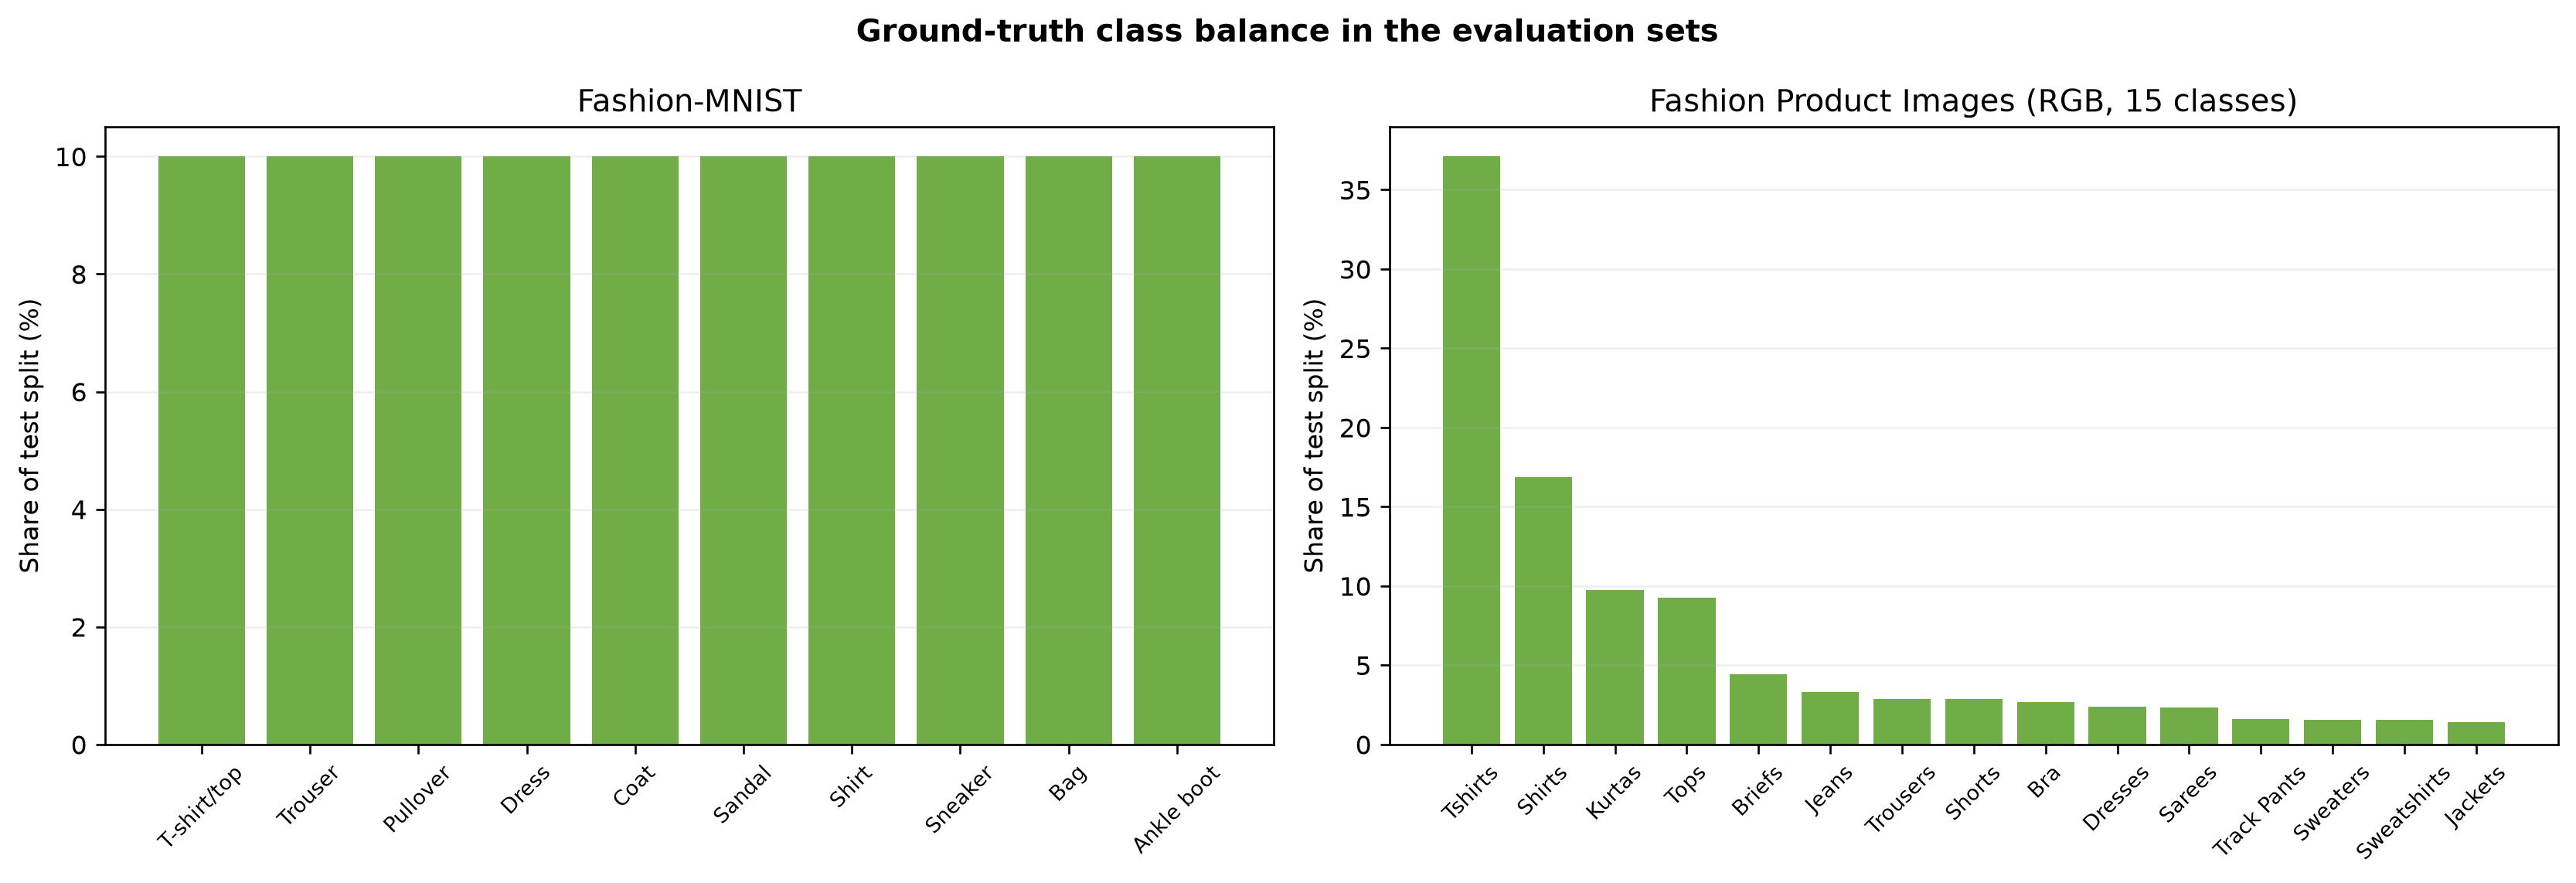
\includegraphics[width=\linewidth]{figures/dataset_class_balance.png}
  \small (b) Test-set class balance
\end{minipage}
\caption{Evaluator reliability and dataset imbalance.}
\end{figure}

\clearpage
\section{Distribution, Convergence, and Compute Diagnostics}
\label{app:diagnostics}
\begin{figure}[ht]
  \centering
  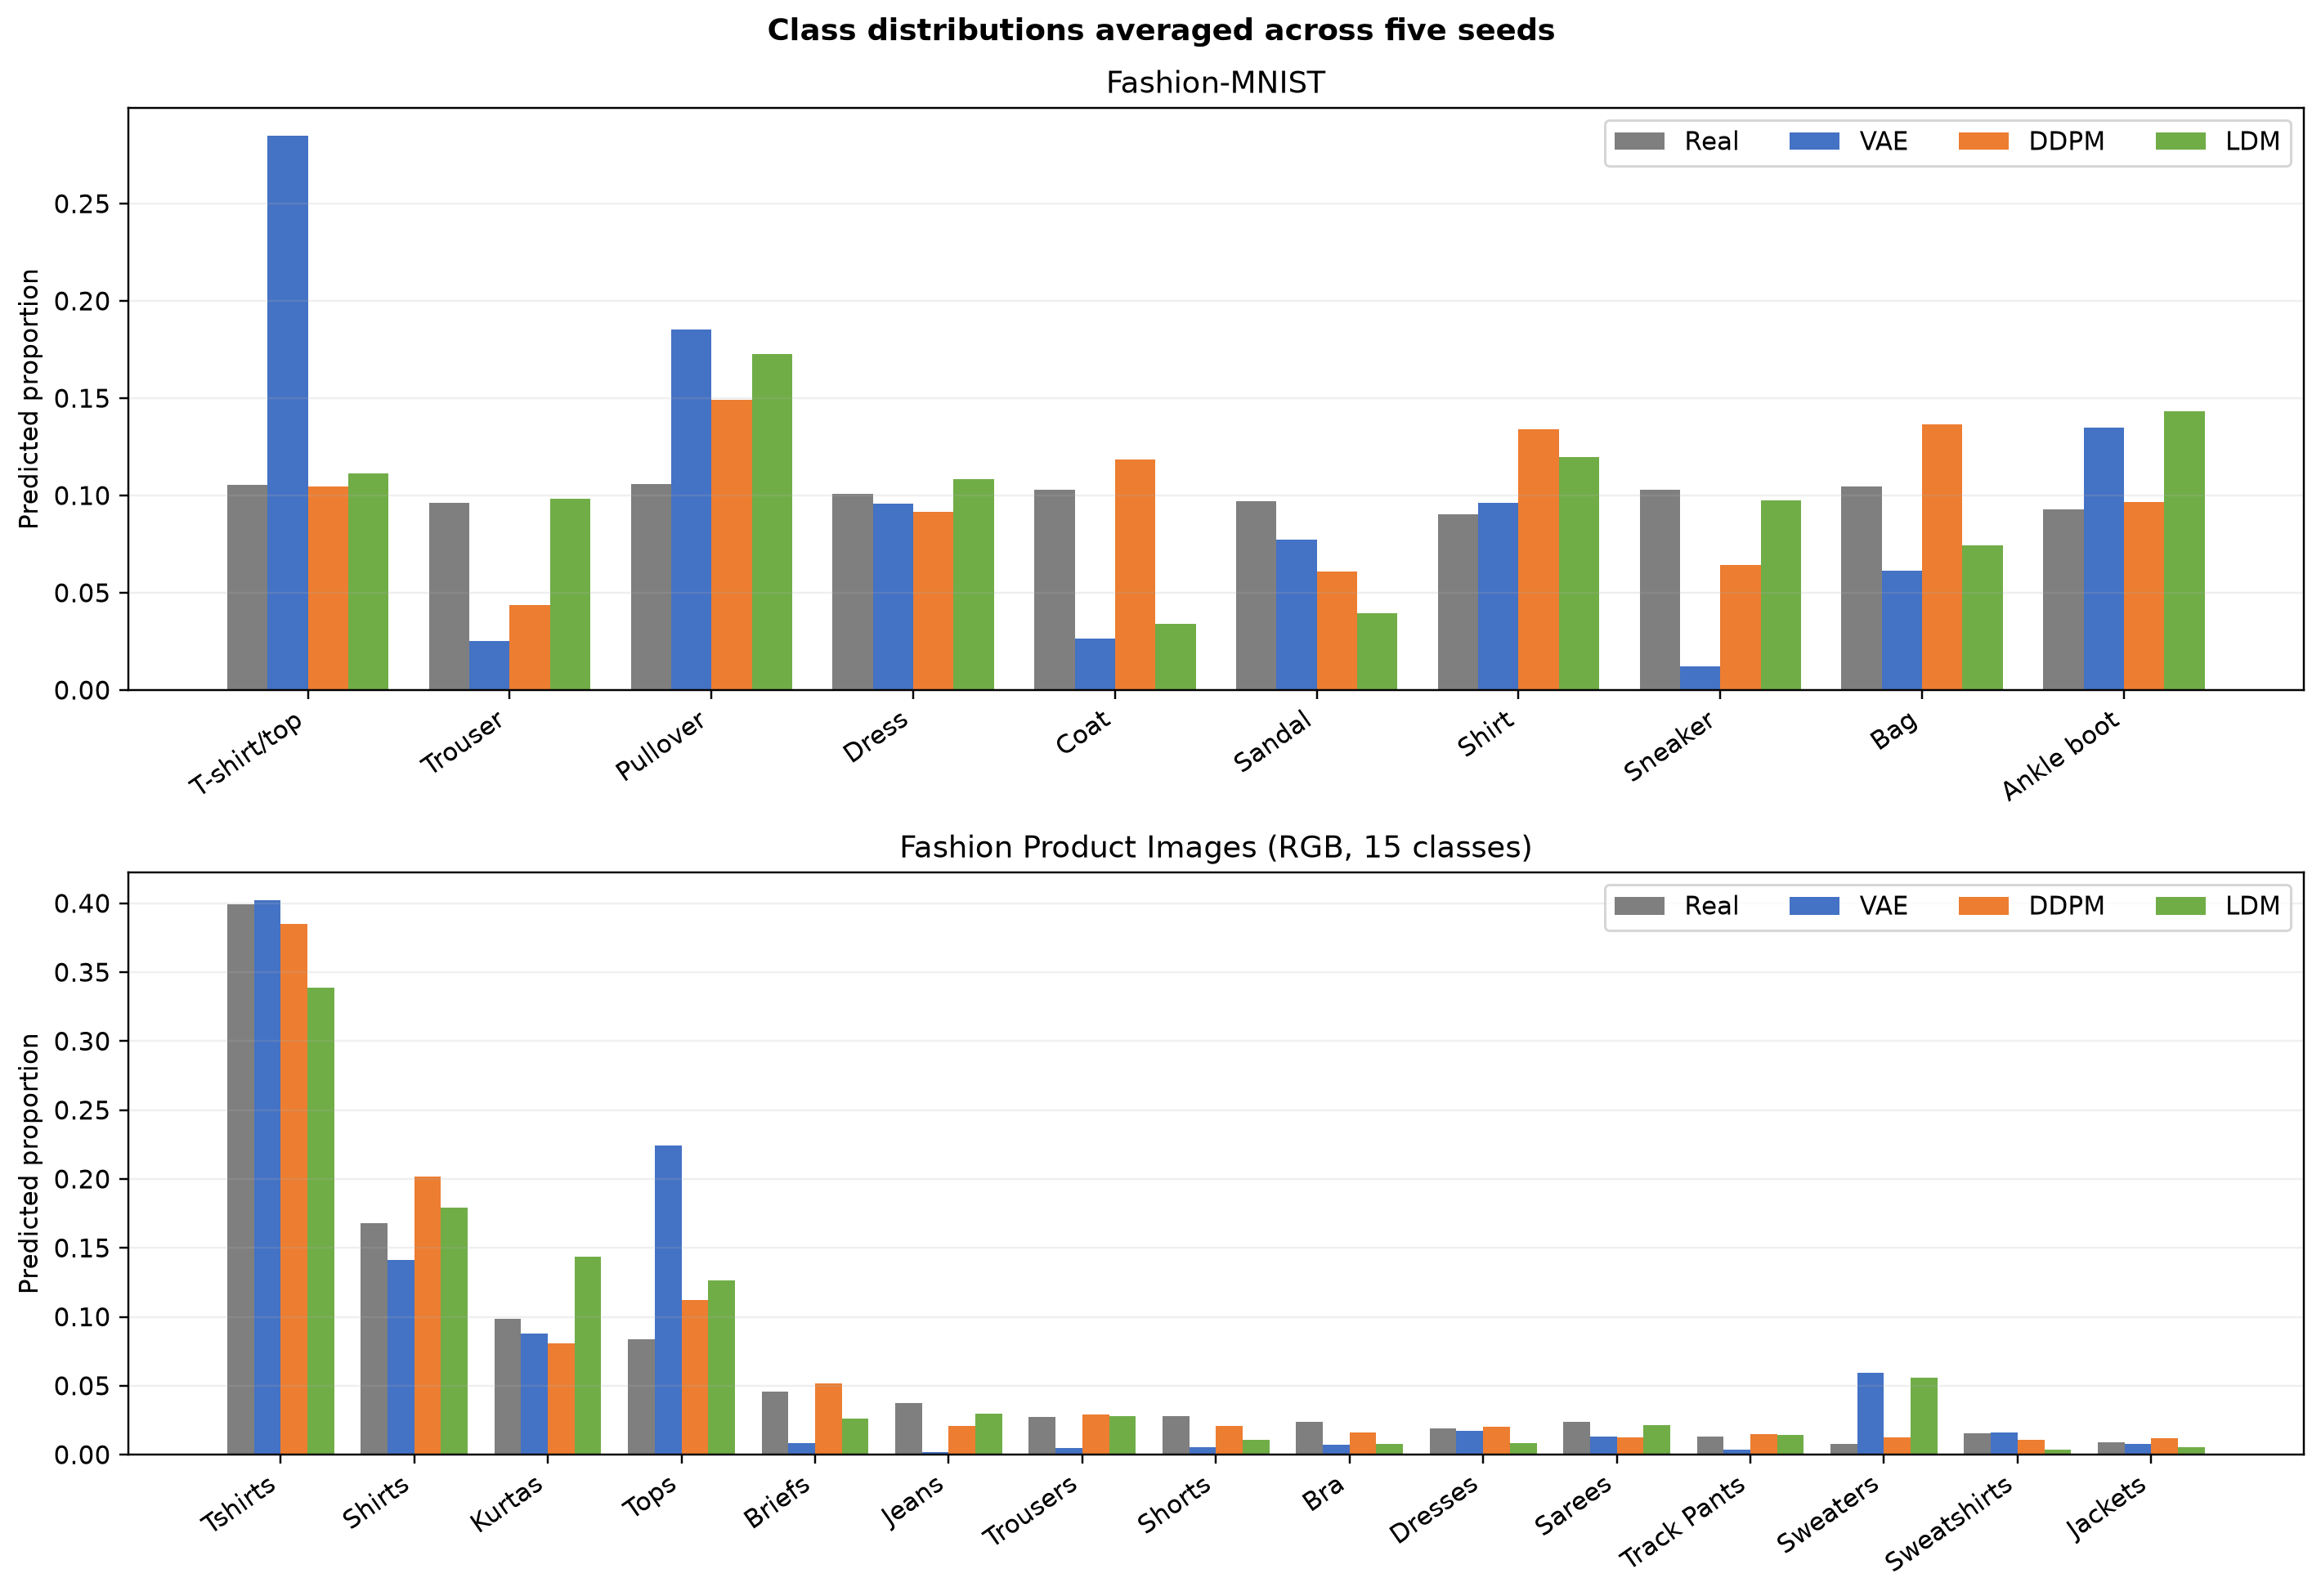
\includegraphics[width=0.98\linewidth]{figures/class_distributions.png}
  \caption{Predicted class distributions averaged over five seeds. DDPM most closely follows the real evaluator distribution.}
\end{figure}

\begin{figure}[ht]
\centering
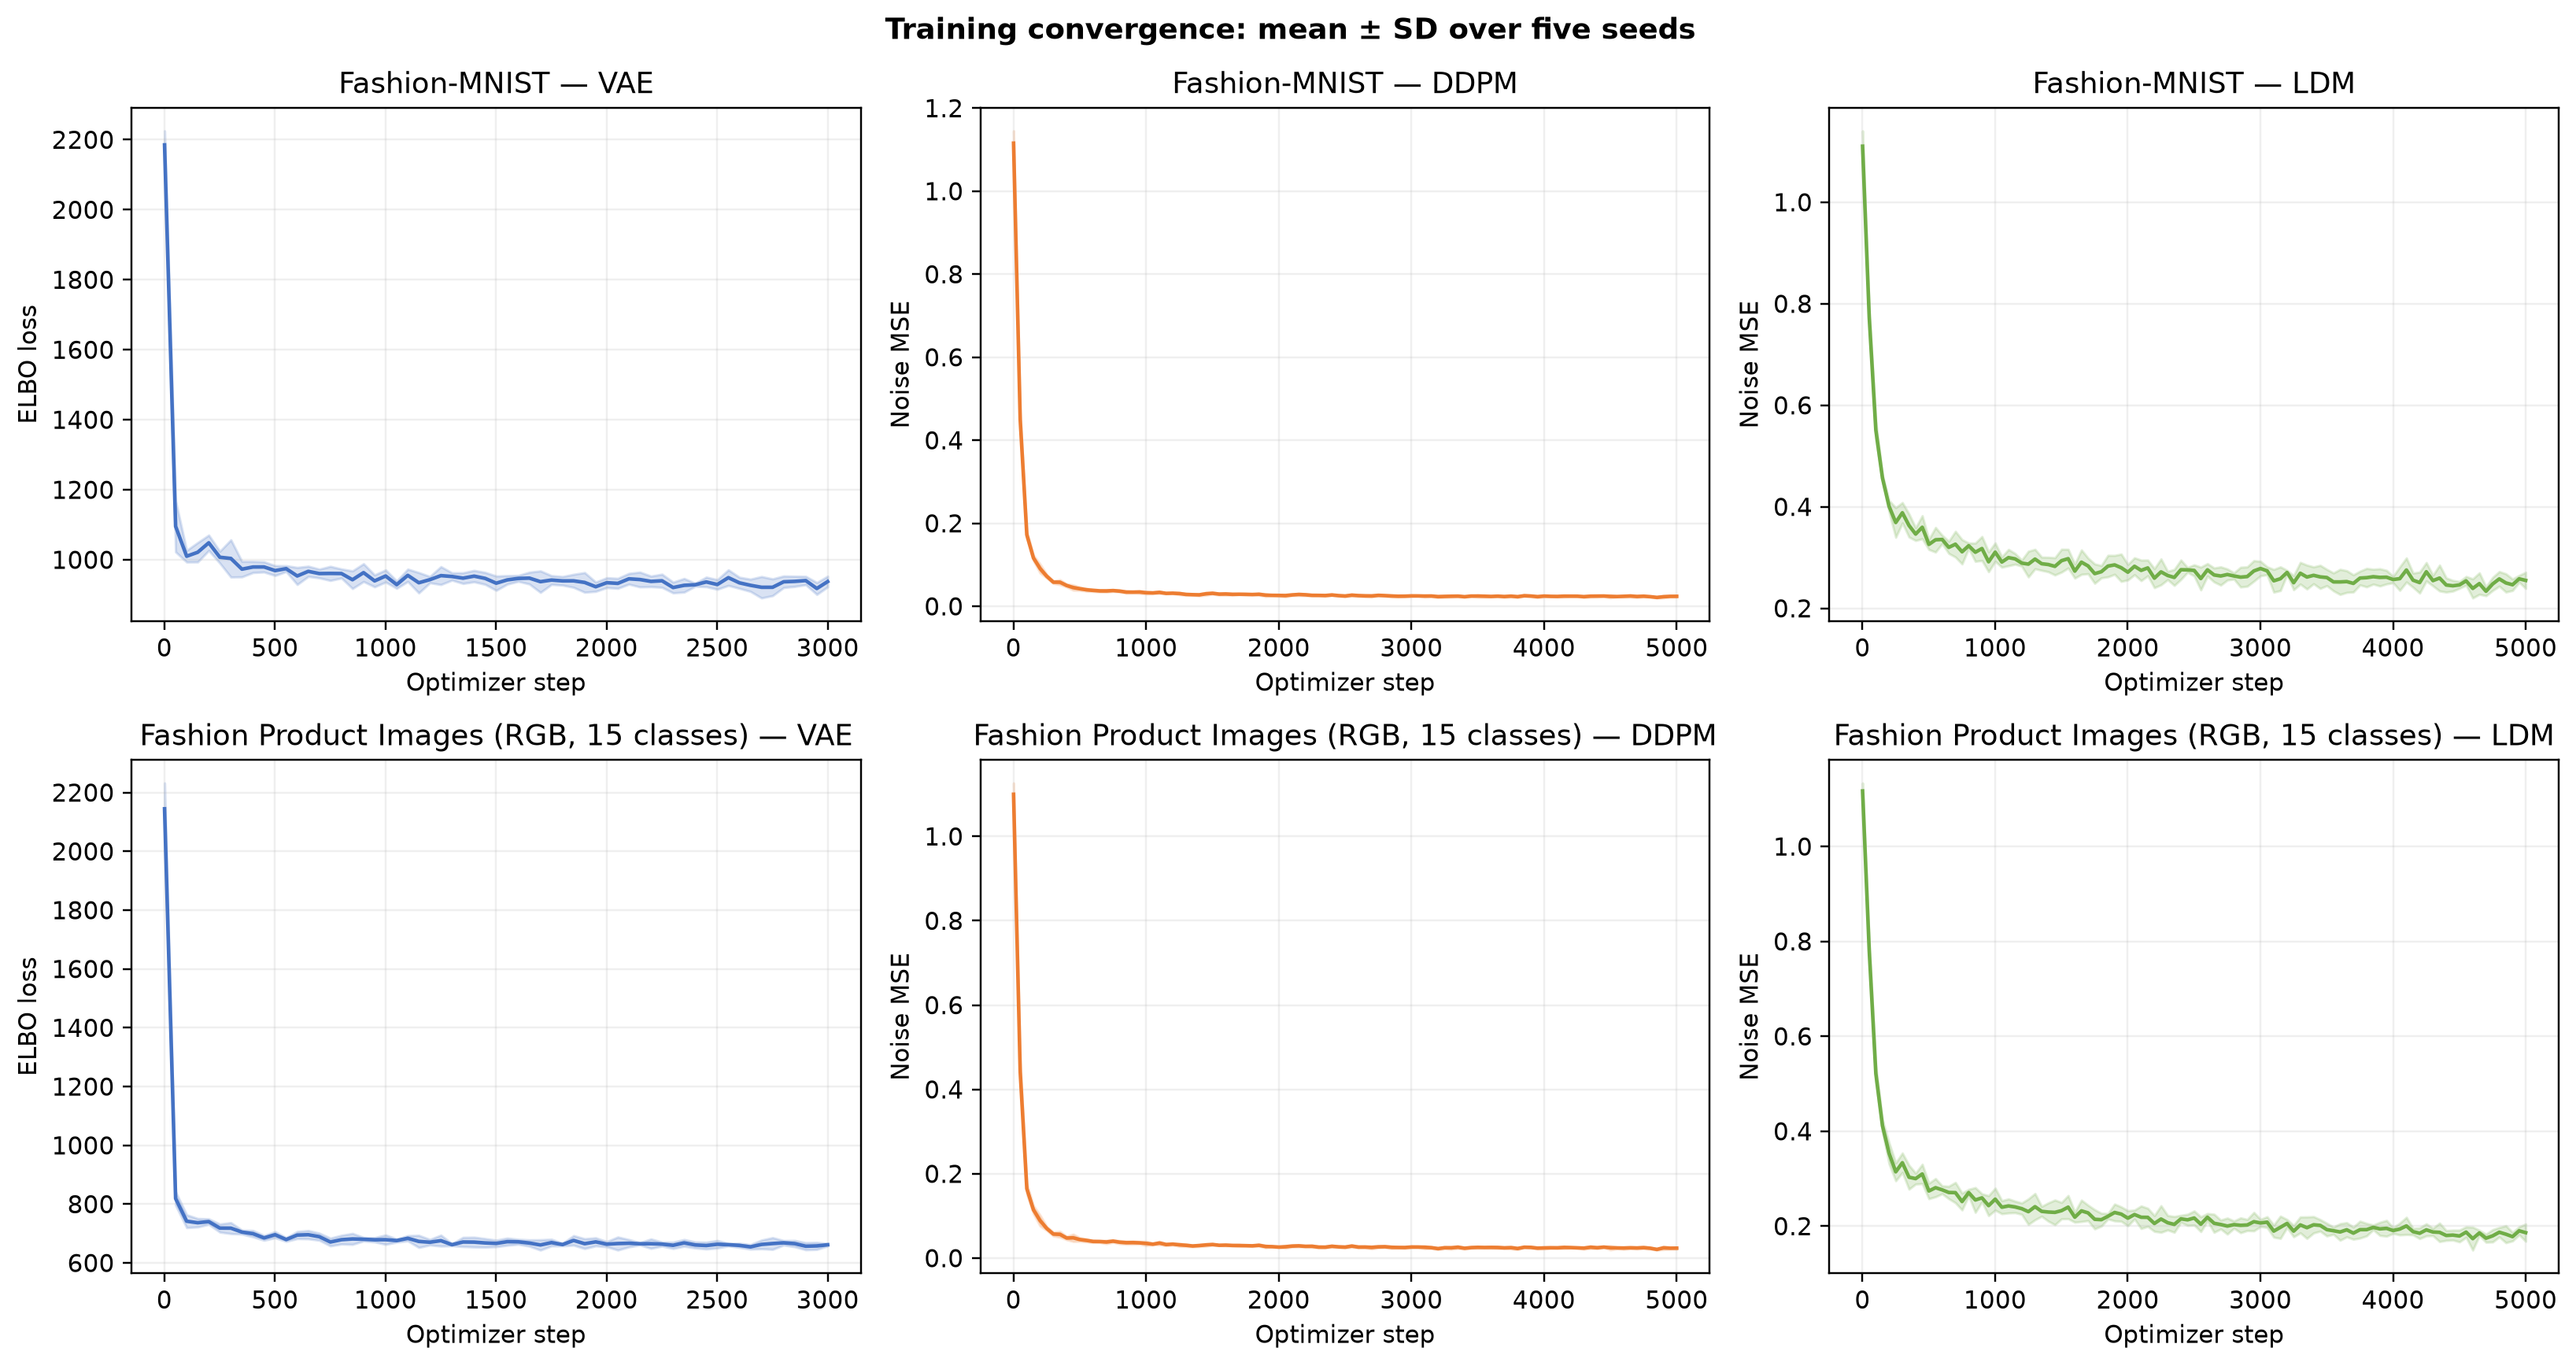
\includegraphics[width=0.78\linewidth]{figures/training_curves.png}
\caption{Mean $\pm$ SD optimization curves over five seeds. Loss magnitudes are not comparable across objectives.}
\end{figure}

\begin{figure}[ht]
\centering
\begin{minipage}{0.49\linewidth}
  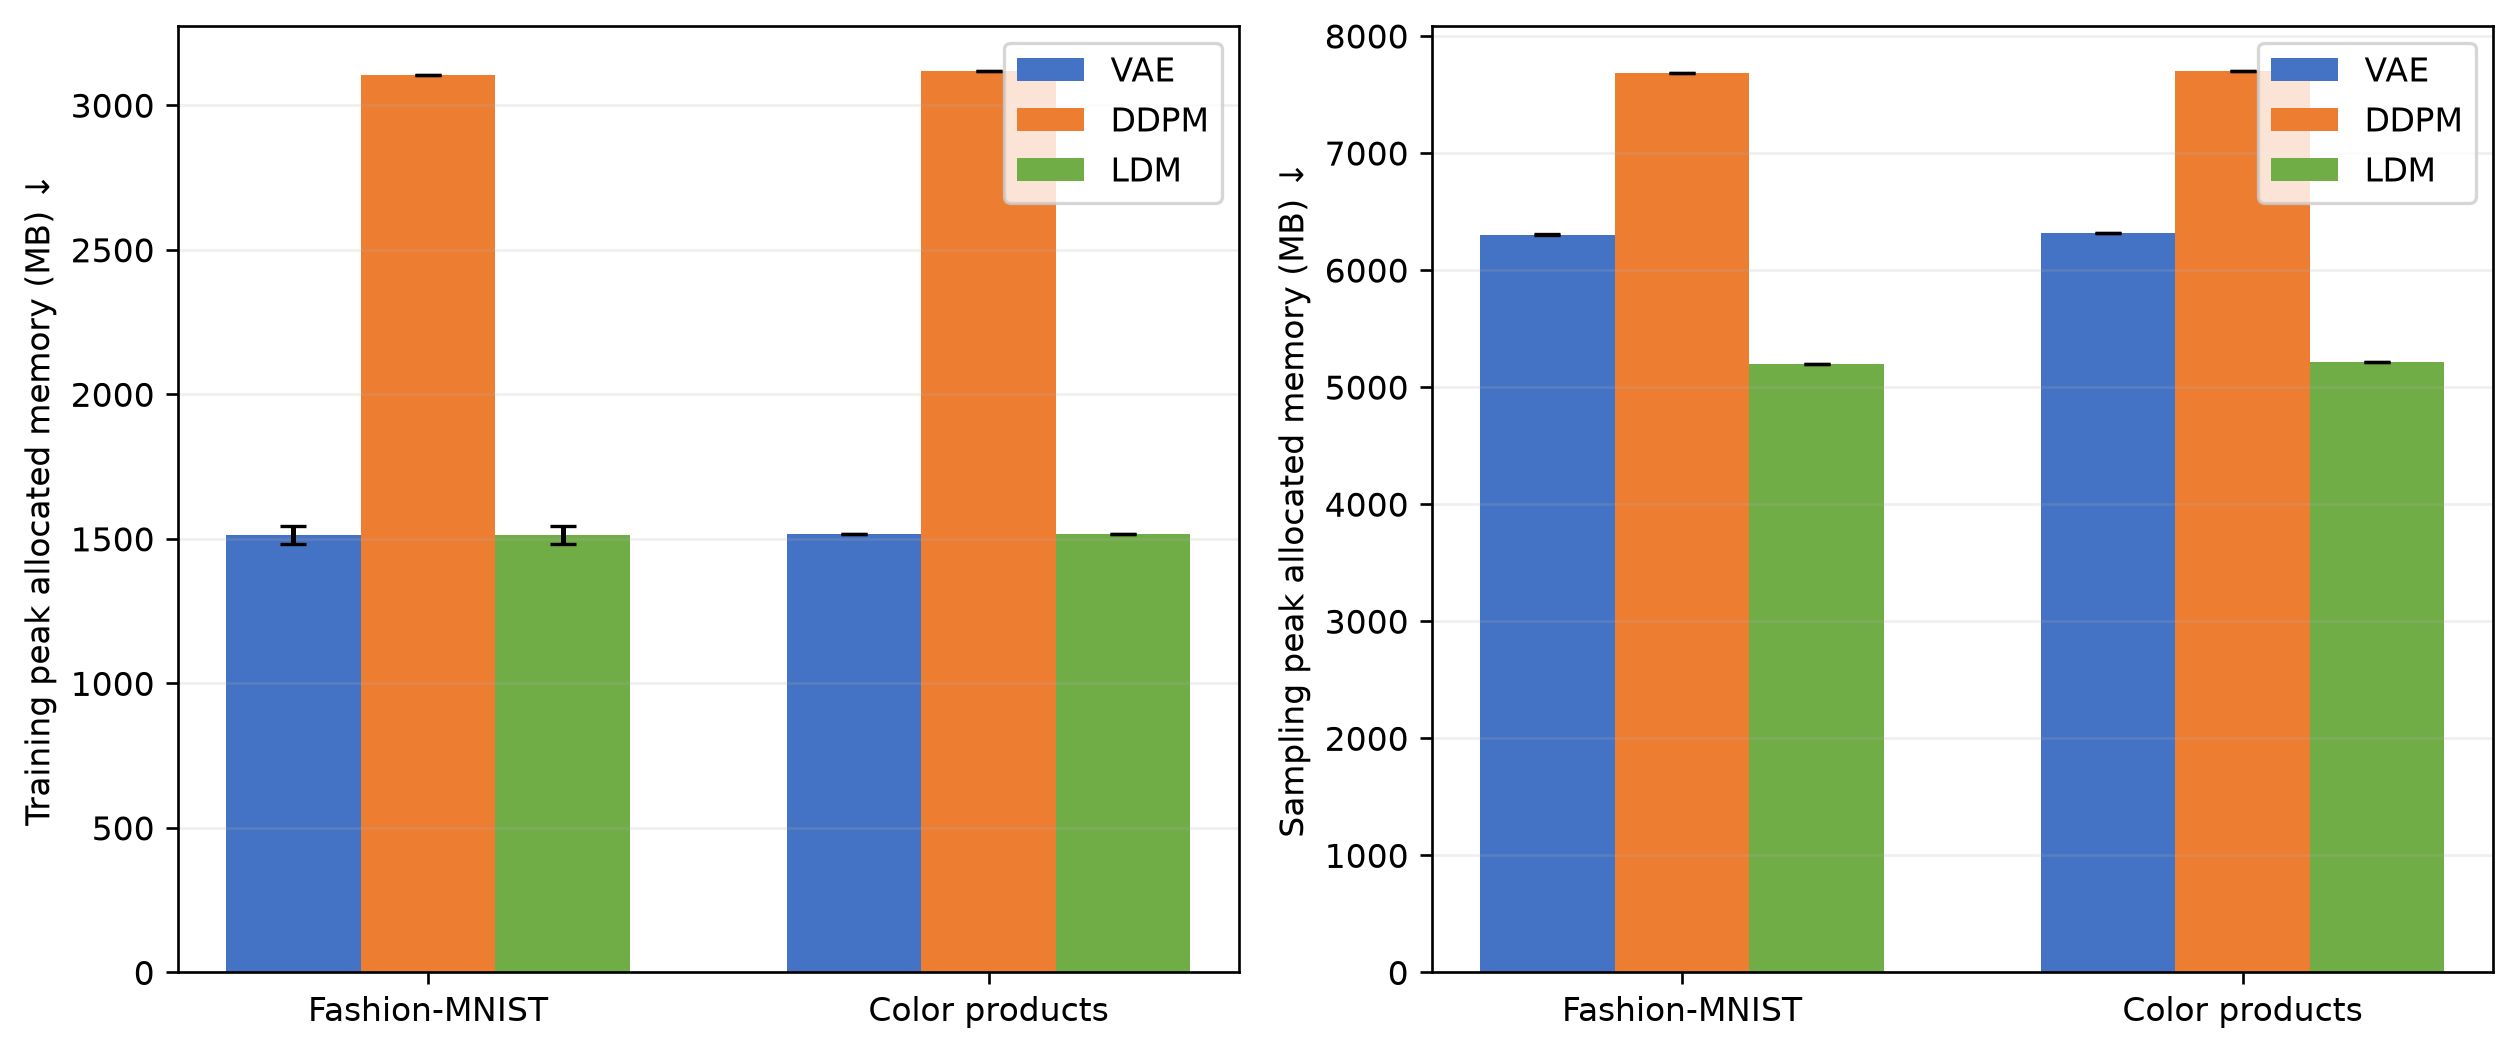
\includegraphics[width=\linewidth]{figures/memory_breakdown.png}
  \small (a) Training and sampling memory
\end{minipage}\hfill
\begin{minipage}{0.49\linewidth}
  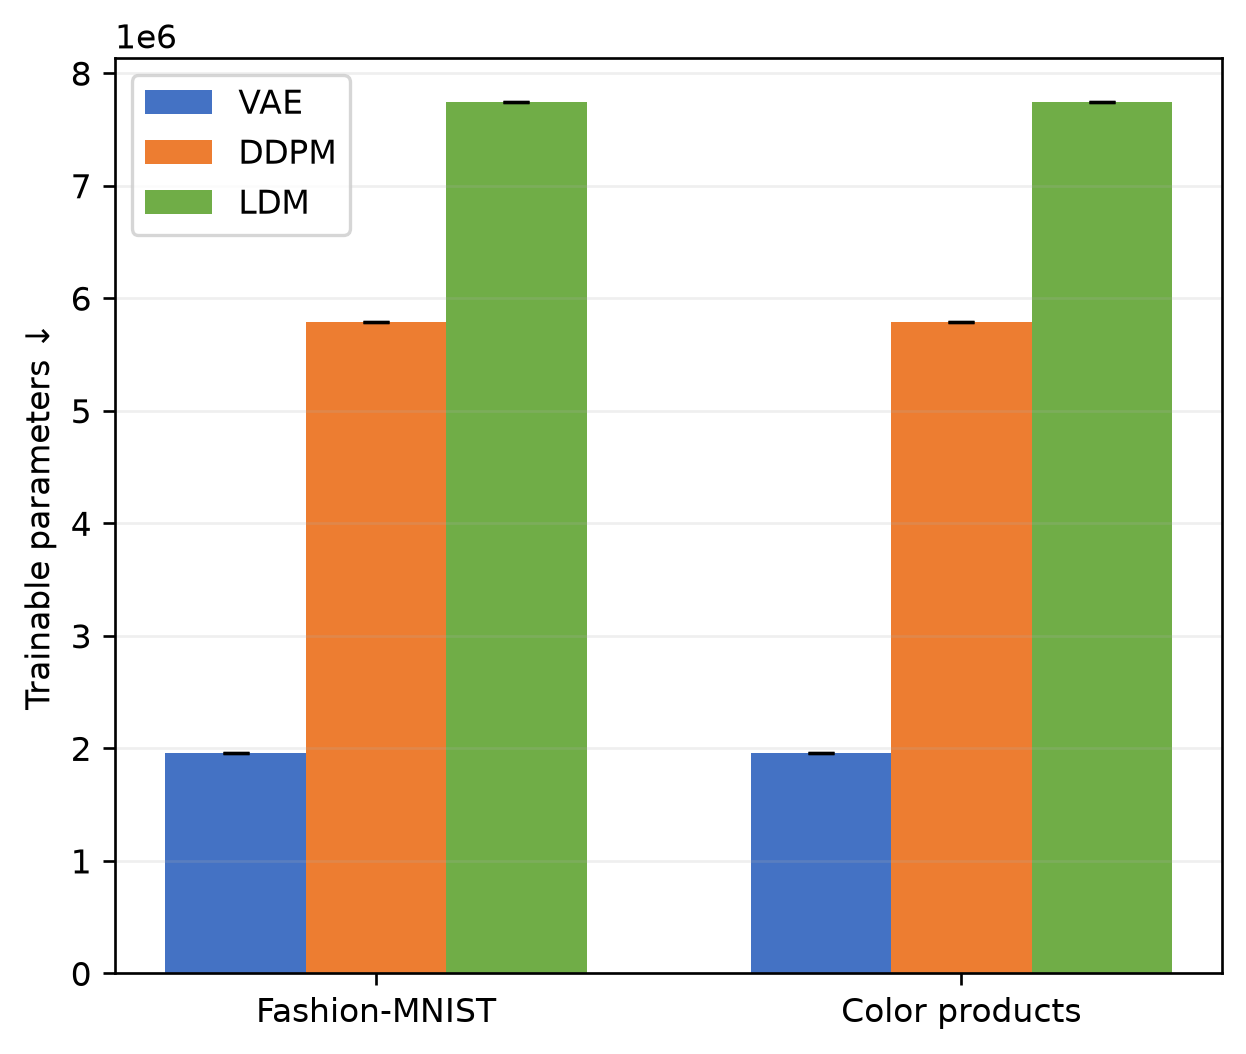
\includegraphics[width=\linewidth]{figures/model_size.png}
  \small (b) Complete-system parameters
\end{minipage}
\caption{Supporting resource diagnostics. The report package also contains all 30 per-seed metric rows and complete mean/SD tables in machine-readable CSV format.}
\end{figure}

\end{document}
